% MolDStruct MC/MD reference manual.  Build: tectonic manual.tex  (or pdflatex twice)
\documentclass[11pt,a4paper,openany]{report}
\usepackage[margin=2.5cm]{geometry}
\usepackage{amsmath,amssymb,bm}
\usepackage{booktabs,array,tabularx,longtable}
\usepackage{graphicx,caption}
\usepackage{xcolor}
\usepackage{float}
\usepackage{listings}
\usepackage{tikz}
\usetikzlibrary{arrows.meta,positioning}
\usepackage{enumitem}
\usepackage[colorlinks=true,linkcolor=blue!50!black,citecolor=green!35!black,urlcolor=blue!50!black]{hyperref}

\definecolor{codebg}{RGB}{247,246,242}
\definecolor{codecomment}{RGB}{110,108,100}
\lstset{basicstyle=\ttfamily\footnotesize, backgroundcolor=\color{codebg}, frame=single,
  rulecolor=\color{black!15}, framesep=4pt, xleftmargin=6pt, xrightmargin=6pt, columns=fullflexible,
  keepspaces=true, breaklines=true, showstringspaces=false, aboveskip=8pt, belowskip=8pt,
  commentstyle=\color{codecomment}\itshape}
\setlist{itemsep=2pt, topsep=4pt}
\emergencystretch=2em

% long file and option names may break after an underscore
\let\oldunderscore\_
\renewcommand{\_}{\oldunderscore\allowbreak}
\newcommand{\code}[1]{\texttt{#1}}
\newcommand{\opt}[1]{\texttt{#1}}            % an mdp option
\newcommand{\env}[1]{\texttt{#1}}            % an environment variable
\newcommand{\file}[1]{\texttt{#1}}
\newcommand{\dd}{\mathrm{d}}
\newcommand{\kc}{k_{\mathrm C}}
\newcommand{\Kmat}{\mathsf K}
\newcommand{\vect}[1]{\bm{#1}}

\title{\Huge MolDStruct MC/MD\\[8pt]
  \Large Hybrid Monte Carlo / molecular dynamics for X-ray induced\\ ionization and Coulomb explosion\\[18pt]
  \large Reference manual}
\author{Biophysics group, Uppsala University}
\date{October 2026 \\[4pt] \small model version: tpr format 79}

\begin{document}
\maketitle
\tableofcontents

\chapter{Introduction}
\label{ch:intro}

MolDStruct MC/MD simulates what happens to a biomolecule, or any small system of light atoms, when it is hit by an
intense femtosecond X-ray pulse.
The pulse ionizes the atoms, the released electrons partly escape and partly stay trapped, the sample charges up and
explodes, and the ions fly apart in directions that still carry information on the original structure.
The model follows all of this in one simulation: the electronic state of every atom, the electrons released, and the
nuclear motion.

It is part of the MolDStruct toolbox and is built on GROMACS~4.5.4~\cite{pronk2013}, extended with an ionization
module.
Everything GROMACS does still works the same way; the ionization model is switched on with \code{mdrun -ionize} and
controlled by \opt{mcmd-*} options in the \file{.mdp} file.

\section{The model in one page}

\begin{description}
  \item[Atoms] are classical particles that also carry an electronic configuration: the number of electrons in their
    K, L and M shells.
    Each configuration has a charge, and the charges enter the force field.
  \item[Electronic transitions] (photoionization by the pulse, Auger--Meitner decay, fluorescence) change those
    configurations.
    They are sampled every MD step by kinetic Monte Carlo from tabulated rates and cross sections
    (Chapter~\ref{ch:atomic}).
  \item[Charge transfer] moves electrons between nearby atoms when a classical over-the-barrier criterion allows it
    (Chapter~\ref{ch:ct}).
  \item[The force field] is modified so that ionized atoms lose their chemical bonds: bonded terms fade out with the
    charge, bonds break irreversibly, and the Coulomb interactions between bonded neighbours are restored
    (Chapter~\ref{ch:ff}).
  \item[Released electrons] either escape or are trapped by the growing positive charge.
    The trapped ones form a hot electron cloud, described as a continuous density in thermal equilibrium with the ions:
    a Poisson--Boltzmann problem solved on a three-dimensional grid every 0.2\,fs (Chapter~\ref{ch:pb}).
    The cloud screens the ions, pulls on them, decides which new electrons escape, and evaporates as the sample
    expands.
  \item[Electron--ion collisions] in the cloud ionize further (Chapter~\ref{ch:coll}).
  \item[Atomic data] (energies, rates and cross sections per configuration) are computed at start-up from a
    screened-hydrogenic shell model, or read from plain-text tables, which can be generated with XATOM (open source)
    or from CRETIN models (Chapter~\ref{ch:data}).
\end{description}

With \opt{mcmd-electrons = none} the electron cloud is switched off: every released electron leaves, and the model is
the original MolDStruct model~\cite{ostlin2018}.

\section{How this manual is organized}

Chapter~\ref{ch:start} gets a first run going.
Chapters~\ref{ch:atomic}--\ref{ch:coll} describe the physics, each with the options that control it.
Chapter~\ref{ch:data} specifies the atomic data, Chapter~\ref{ch:output} every output file.
Chapters~\ref{ch:mdp} and~\ref{ch:env} are the reference: every mdp option and every diagnostic environment variable.
The appendices cover the numerics of the electron model (Appendix~\ref{app:numerics}), parallel runs
(Appendix~\ref{app:parallel}), validation and limitations (Appendix~\ref{app:validation}), and units, the source
files and the version history (Appendix~\ref{app:misc}).

Basic knowledge of GROMACS is assumed; see the GROMACS documentation for anything not specific to the ionization
model.

\section{Conventions}

Inside the model energies are in eV, lengths in nm, and times in ps as in GROMACS --- except the pulse options and
the electron-model intervals, which are in \textbf{femtoseconds}.
Charges are in units of $e$.
A configuration is written \code{K L M}, e.g.\ \code{2 4 0} for neutral carbon and \code{1 4 0} for carbon with a
K-shell hole.
Potentials are \emph{potential energies of an electron}, in eV.

\section{Citing}

If you use MolDStruct MC/MD, please cite the MolDStruct paper (to be added on publication), and GROMACS~4.5
\cite{pronk2013}.
The built-in atomic data follow Scott and Hansen~\cite{scott2010}; if you use atomic data generated with XATOM, cite
XATOM~\cite{jurek2016}.

\chapter{Getting started}
\label{ch:start}

\section{Installation}

The build is that of GROMACS~4.5.4 with CMake.
FFTW~3 (single precision) is required; it is also what the electron model uses for its grid convolutions.
\begin{lstlisting}
cd gromacs-4.5.4-MCMD
mkdir build && cd build
cmake .. -DCMAKE_INSTALL_PREFIX=/path/to/install
make -j8 install
\end{lstlisting}
Use the \code{grompp} of this build to write run inputs: the \file{.tpr} format carries the \opt{mcmd-*} options
(format 80), which a stock GROMACS cannot read (and an older stock GROMACS tool would silently misread).
Set \env{GMXLIB} to the build's \file{share/top} if the force fields are not found.

\section{The example}

\file{example/} holds a complete run: hen egg-white lysozyme (PDB 1AKI, 1960 atoms) in vacuum, exploded by a
Gaussian pulse of $10^{11}$ photons at 1000\,eV, 2.94\,fs FWHM, focused to 100\,nm.
\begin{lstlisting}
cd example
pdb2gmx -f 1aki.pdb -ff charmm27 -water none
grompp  -f exp.mdp -c conf.gro -p topol.top -o explode.tpr
mdrun   -deffnm explode -v -nt 4 -pd -ionize
\end{lstlisting}
(\file{run\_example.sh} does the same.)
The run is 15\,000 steps of 2\,as, i.e.\ 30\,fs with the pulse peaking at $t=0$, and takes about 10 minutes on 4
threads.
No atomic data files are needed: the module computes them for 1000\,eV at start-up (Section~\ref{sec:builtin}).
The model is the default one; the ``Model'' block of \file{exp.mdp} lists its main options.

\paragraph{What to expect.}
\opt{mcmd-seed = -1} draws a new random seed every run, so the numbers differ by about a percent between runs.
Roughly:
\begin{itemize}
  \item every atom ends up ionized; the mean charge is about 3.5 per atom (hydrogen fully stripped, carbon $\sim$5.4,
    nitrogen $\sim$6.2, oxygen $\sim$7.1, sulfur $\sim$13.6);
  \item about 4000 photoionizations, 800 Auger decays, 2100 electron-impact ionizations and 820 charge transfers;
  \item of the $\sim$6900 electrons released, $\sim$1350 have escaped and $\sim$5600 are still trapped at 30\,fs, at a
    temperature of $\sim$18\,eV; the radius of gyration has grown 3.6-fold, to $\sim$5.7\,nm.
\end{itemize}
\code{tools/mcmd\_output.py plot} draws an overview of the whole run (Section~\ref{sec:viewer}).

\section{The run summary}
\label{sec:summary}

At start-up \code{mdrun} prints a summary of what the module will do, and writes the same block to \file{md.log}
(after GROMACS's own parameter listing): the system, the pulse, the run length and seed, the atomic data found, every
process and whether it is on, and the output.
For the example:
\begin{lstlisting}
==================================================================================
 MolDStruct MC/MD
 System        1960 atoms (H 959, C 613, N 193, O 185, S 10), all neutral at the start
 Pulse         1000 eV, Gaussian, FWHM 2.9435 fs, peak at 0 fs, 1e+11 photons into 100 nm
               (1.27e+13 photons/um^2); bandwidth 0.003
 Run           15000 steps x 2 as = 30 fs; seed 3104721958 (chosen at start, mcmd-seed = -1); 4 ranks
 Atomic data   built in: screened-hydrogenic shells (K, L, M) at 1000 eV, mcmd-atomic-data = hydrogenic
               (written to ./simulation_output/Atomic_data)

 Processes
   photoionization, Auger, fluorescence     on (always)
   charge transfer                          on   hydrogen donors only, H-H off, downhill off
   trapped electrons (Poisson-Boltzmann)    on   mcmd-electrons = pbgrid
       grid                                 s_e 0.25 nm, 2.5 cells/s_e, box <= 3 R, <= 384 cells,
                                            solve every 0.2 fs, Newton tol 0.01
       evaporation                          on
   ion-ion forces                           all pairs
   electron-impact ionization               on   Lotz, built in (mcmd-coll-data = lotz)
   three-body recombination                 off
   collisional excitation                   off
   field ionization                         off

 Output        simulation_output/: transitions.bin (mcmd-detailed-output = 1), charges_over_time.bin every 500 steps;
               autostop off
 Settings      all at the validated production values
==================================================================================
\end{lstlisting}
Settings outside the validated model are listed as warnings instead of the last line --- an MD step above 2\,as, a
PB solver coarser than the converged settings, a non-default smoothing, three-body recombination, collisional
excitation, H--H charge transfer, all pairs above 10\,000 atoms, harmonic bonds that cannot break, a pulse without
photons.
The run goes on; the warnings say that the result is not covered by the validation of
Appendix~\ref{app:validation}.

\section{Running your own system}

\begin{enumerate}
  \item Prepare the system as for any vacuum GROMACS run: \code{pbc = no}, no pressure or temperature coupling during
    the explosion.
    Equilibrate it beforehand without \code{-ionize}.
  \item Set \code{morse = yes} so that \code{grompp} turns the bonds into Morse potentials, which can break
    (Chapter~\ref{ch:ff}).
  \item Use \code{dt = 0.000002} (2\,as) and the pulse options \opt{mcmd-pulse-*} (Chapter~\ref{ch:mdp}); note that
    the pulse times are in fs.
  \item The atomic data are computed for the photon energy of the pulse (H to Ar except He); for other data supply
    \file{Atomic\_data/} and set \opt{mcmd-atomic-data = files} (Chapter~\ref{ch:data}).
  \item Run \code{mdrun -ionize}, with \code{-nt N -pd} for more than one thread (Appendix~\ref{app:parallel}).
\end{enumerate}
Ion-ion Coulomb interactions are taken care of by \opt{mcmd-pb-long-range = auto}: all pairs up to 10\,000 atoms,
a 2\,nm cutoff plus the long-range field from the grid above (\code{grompp} sets the cut-offs and says so).

\section{Reproducible runs and continuation}
\label{sec:seed}

The Monte Carlo draws come from a random seed.
With \opt{mcmd-seed = -1} (the default) it is drawn from the clock and the process id at start-up, so every run is
a different realization --- which is what an ensemble needs.
The seed is printed in the summary; set \opt{mcmd-seed} to it to repeat a run exactly (on the same number of
ranks, Appendix~\ref{app:parallel}).
Give every member of an ensemble its own seed, or leave it at $-1$.

Runs can be continued from a GROMACS checkpoint with \code{mdrun -cpi}.
At every checkpoint the module writes \file{simulation\_output/mcionize\_state.bin} (the previous one kept as
\file{mcionize\_state\_prev.bin}): the electronic configurations, the electron cloud's state, the random streams, the
reference radius the expansion is measured against, and the length of every output file.
On restart the state of the checkpoint's step is read back, the output files are cut back to that step and appended
to.
The state file is required: the reference radius in particular cannot be recovered from an expanded sample.
To extend a finished run, raise \code{nsteps} with \code{tpbconv -extend} and continue with \code{-cpi}.

\section{The regression test}

\file{test/regression.sh} runs the example for 300 steps with a pinned seed in two cases --- \code{none} (no
electron cloud) and \code{full} (the defaults, on a coarse grid) --- and checks that the event counts match the
stored references exactly and that the charge is conserved.
Then, with \opt{mcmd-atomic-data = files} on the tables the full case wrote, it checks that they reproduce the run
bit for bit, that a run without \code{-ionize} writes no ionization output, that the total energies are required
exactly when charge transfer or collisions need them, and that the run is unchanged without the statistical weights.
It takes under a minute; \code{--update} regenerates the references after a deliberate change of the physics.
The references are only meaningful for the build and machine that wrote them.

\chapter{The atomic model}
\label{ch:atomic}

\section{Electronic states}

The electronic state of an atom is its \emph{shell configuration}: three integers \code{K L M}, the number of
electrons in the $n=1,2,3$ shells (capacities 2, 8 and 18).
There are no subshells and no terms or levels within a configuration; whatever an atomic-structure code resolves
is summed or averaged per configuration when the data are generated (Chapter~\ref{ch:data}).
An atom starts in its element's ground configuration (table~\ref{tab:elements}).
Its charge in the MD is $q = Z - (K+L+M)$: at the first step the module replaces the force field's partial charges by
these integer ionization charges (all zero at the start), and every transition changes the configuration and the
charge.

An atom's element is the one whose standard atomic weight is nearest to its mass, within 0.5 (so argon, 39.948, and
calcium, 40.078, are told apart):

\begin{table}[H]
\centering\small
\begin{tabular}{@{}lrrl@{\quad}lrrl@{\quad}lrrl@{}}
\toprule
element & mass & $Z$ & ground & element & mass & $Z$ & ground & element & mass & $Z$ & ground \\
\midrule
H  & 1.008  & 1 & \code{1 0 0} & F  & 18.998 & 9  & \code{2 7 0} & S  & 32.06  & 16 & \code{2 8 6} \\
Li & 6.94   & 3 & \code{2 1 0} & Ne & 20.180 & 10 & \code{2 8 0} & Cl & 35.45  & 17 & \code{2 8 7} \\
Be & 9.0122 & 4 & \code{2 2 0} & Na & 22.990 & 11 & \code{2 8 1} & Ar & 39.948 & 18 & \code{2 8 8} \\
B  & 10.81  & 5 & \code{2 3 0} & Mg & 24.305 & 12 & \code{2 8 2} & Ca & 40.078 & 20 & \code{2 8 10}$^\ast$ \\
C  & 12.011 & 6 & \code{2 4 0} & Al & 26.982 & 13 & \code{2 8 3} & Fe & 55.845 & 26 & \code{2 8 16}$^\ast$ \\
N  & 14.007 & 7 & \code{2 5 0} & Si & 28.085 & 14 & \code{2 8 4} & Ni & 58.693 & 28 & \code{2 8 18}$^\ast$ \\
O  & 15.999 & 8 & \code{2 6 0} & P  & 30.974 & 15 & \code{2 8 5} & I  & 126.904 & 53 & \code{2 8 18}$^{\ast\ast}$ \\
\bottomrule
\end{tabular}
\caption{Elements the module knows (\code{mcmd\_elements[]} in \file{atomic\_data.c}); H to Ar have built-in data.
$^\ast$\,The 4s electrons are counted in M; only with \opt{mcmd-atomic-data = files}.
$^{\ast\ast}$\,A placeholder: right for the force field, not for the ionization physics.
Deuterium (mass 2) is hydrogen.  Helium is left out: an atom of mass $\sim$4 is far more likely a heavy hydrogen
(\code{pdb2gmx -heavyh}, mass repartitioning) and is refused rather than taken as helium.}
\label{tab:elements}
\end{table}
A new element needs a row in that table (mass, symbol, ground configuration) and, above argon or for files, its
atomic data.

\section{Transitions}

Three processes are tabulated per configuration, each with its final configuration:
\begin{description}
  \item[Photoionization] (type 2) removes one electron from a shell.
    The table gives the cross section $\sigma$ (cm$^2$) at the photon energy; the rate is $\sigma I(t)$ with the pulse
    flux $I(t)$ below.
  \item[Auger--Meitner decay] (type 0) fills a hole from an outer shell and ejects a second electron: the atom loses
    one electron.
    The table gives the rate (s$^{-1}$).
  \item[Fluorescence] (type 1) fills a hole from an outer shell and emits a photon, which leaves; the charge does not
    change.
\end{description}
Charge transfer (Chapter~\ref{ch:ct}) and, with the electron cloud, collisional ionization
(Chapter~\ref{ch:coll}) are added to these.

\section{The pulse}

The pulse is Gaussian in time, with peak time $t_0$ (\opt{mcmd-pulse-peak-time}), full width at half maximum
$\tau$ (\opt{mcmd-pulse-fwhm}), $N_{\mathrm{ph}}$ photons (\opt{mcmd-pulse-photons}) in a focal spot of
diameter $d$ (\opt{mcmd-pulse-focal-diameter}), uniform over the sample:
\begin{equation}
  I(t) = \frac{N_{\mathrm{ph}}}{\pi (d/2)^2}\,\frac{1}{\sigma_t\sqrt{2\pi}}\,
         \exp\!\Big[-\frac{(t-t_0)^2}{2\sigma_t^2}\Big],\qquad \sigma_t = \frac{\tau}{2\sqrt{2\ln 2}},
\end{equation}
in photons cm$^{-2}$\,s$^{-1}$.
The fluence $N_{\mathrm{ph}}/(\pi d^2/4)$ is what sets the ionization; the example's $10^{11}$ photons into 100\,nm
are $1.27\times10^{13}$ photons/\textmu m$^2$.
The photon energy (\opt{mcmd-pulse-photon-energy}) only enters through the atomic data, which are computed for it
(built in) or must be generated for it (files),
and through the energy of the photoelectrons.
\opt{mcmd-pulse-bandwidth} (relative FWHM, default 0.003) gives each photoelectron a Gaussian jitter of that width
in its energy, which matters only for the escape test near threshold; the cross sections are those of the nominal
energy.

\section{The Monte Carlo step}

Every MD step $\Delta t$, every atom is advanced by a first-reaction kinetic Monte Carlo~\cite{gillespie1976}:
for each transition available from its current configuration a waiting time $\delta t = -\ln u / k$ is drawn
($u$ uniform, $k$ the rate, with $I(t)$ for photoionization); the earliest fires if it falls within the time left in
the step; then the atom's new configuration offers new transitions, and the procedure repeats until the step is used
up.
Several transitions can therefore happen to one atom in one step, e.g.\ a K-shell photoionization followed within
femtoseconds by an Auger decay.
The Monte Carlo runs on the master rank from one random stream (seeded by \opt{mcmd-seed},
Section~\ref{sec:seed}), so the sequence of events does not depend on the number of ranks.

\section{The released electrons}

Each photoionization and Auger decay releases an electron, with kinetic energy from the configurations' total
binding energies $T$ (Chapter~\ref{ch:data}):
\begin{equation}
  \varepsilon_{\mathrm{photo}} = E_{\mathrm{ph}} - \big(T_{\mathrm{from}} - T_{\mathrm{to}}\big),\qquad
  \varepsilon_{\mathrm{Auger}} = T_{\mathrm{to}} - T_{\mathrm{from}}.
\end{equation}
For carbon at 1000\,eV a K-shell photoelectron has $\sim$700\,eV and a KLL Auger electron $\sim$260\,eV.
Without the electron cloud (\opt{mcmd-electrons = none}) every electron leaves.
With it, the electron escapes if $\varepsilon$ exceeds the depth of the potential well at its atom, and is trapped in
the cloud otherwise (Section~\ref{sec:escape}).

\chapter{Charge transfer}
\label{ch:ct}

In a charged sample electrons move between atoms: a highly charged ion pulls an electron over the barrier from a
nearby, less charged atom.
The model does this with a classical over-the-barrier criterion (\opt{mcmd-charge-transfer = 1}, the default).

\section{The criterion}

For a pair of atoms of different charge, the less charged one is the donor (charge $Q_D$) and the other the
acceptor ($Q_A$).
The electron goes over the barrier when the pair is closer than
\begin{equation}
  R_{\mathrm{crit}} = \frac{\kc\big(Q_D + 1 + 2\sqrt{(Q_D+1)\,Q_A}\big)}{E_{\mathrm{donor}}},
\end{equation}
with $E_{\mathrm{donor}}$ the binding energy of the donor's outermost electron (\file{energy\_levels\_X.txt}).
Atoms are visited in random order, and each takes the nearest partner that qualifies, within a cutoff of 1.5\,nm
(a cell list keeps the search linear in the number of atoms).

\section{Which shell the electron enters}

Following Boll \emph{et al.}~\cite{boll2022}, the electron enters the acceptor vacancy whose binding energy is closest to
that of the donor orbital it came from.
The binding energy in shell $s$ of configuration $c$ is a difference of total energies,
\begin{equation}
  \varepsilon(c,s) = T(c + e_s) - T(c),
\end{equation}
defined for every shell, also for autoionizing configurations.
This is why \file{total\_energies\_X.txt} is required whenever charge transfer is on.
Only shells up to the ground-state occupation are filled, and a vacancy below an occupied shell (a K hole under a
filled L shell) is skipped: refilling the shell that absorbed the photon would short-circuit the Auger cascade the
rates already describe.

\section{Variants}

\begin{description}
  \item[\opt{mcmd-ct-h-donor-only = 1}] (default): only neutral hydrogen donates, the behaviour of the published
    model.
    Hydrogen barely photoionizes at these photon energies and is stripped early by its neighbours.
  \item[\opt{mcmd-allow-h-ct}] (default 0): allow transfer between two hydrogens.
    This is resonant and moves no net charge; it is off by default and not fully validated.
  \item[\opt{mcmd-charge-transfer-downhill}] (default 0): require the transfer to leave the electron more tightly
    bound, counting the Coulomb energy the pair releases, $(Q_A - Q_D - 1)\kc/R$, by more than $10^{-6}$\,eV.
    On the lysozyme example it changes the number of transfers by an order of magnitude without changing any
    observable: charge transfer saturates, and the extra transfers only reshuffle charge the energetics have already
    fixed.
\end{description}

\section{Scheduling}

The pass over all atoms runs every MD step until nothing has transferred for \opt{mcmd-charge-transfer-idle} steps
(default 2000); it then runs only every \opt{mcmd-charge-transfer-recheck} steps (default 100), and every step again
as soon as a transfer happens.
Because transfer is applied per step rather than at a rate, these two settings change how many transfers happen; they
are not pure performance options.
A negative idle value never goes idle.

\chapter{The modified force field}
\label{ch:ff}

A force field describes a molecule held together by chemical bonds.
Once its atoms are ionized, the electrons that formed those bonds are gone, and the bonded terms would hold the
exploding fragments together with a strength they no longer have.
With \code{mdrun -ionize} the bonded and 1--4 interactions are therefore modified as the atoms charge up
(\file{src/gmxlib/bondfree.c} and \file{src/gmxlib/nonbonded/nonbonded.c}; the switch is the global
\code{moldstruct\_altered\_ff}).
Without \code{-ionize} the force field is that of stock GROMACS.

\section{Charges}

At the first step the module replaces every atom's partial charge by its ionization charge $q = Z-(K+L+M)$, zero for
a neutral atom.
From then on the Coulomb interactions act only between ions, with integer charges that change as the atoms ionize.
The Lennard-Jones interactions are not modified.

\section{The ionization factor}

Every modified bonded term is scaled by the \emph{ionization factor} of the mean charge $\bar q$ of the atoms it
involves:
\begin{equation}
  f(\bar q) = \min\!\big(1,\ \max(1-\bar q,\ 0)\big),
\end{equation}
which is 1 for neutral atoms, falls linearly, and is 0 once the atoms carry on average one charge.
Energies and forces are scaled together, so the scaled terms remain conservative at fixed charge.

\begin{table}[H]
\centering\small
\begin{tabularx}{\textwidth}{@{}l l X@{}}
\toprule
interaction & GROMACS function & modification under \code{-ionize} \\
\midrule
Morse bond & \code{morse\_bonds} & breaks irreversibly at $\beta(r-b_0) > 4$; then removed and replaced by the pair's
  $C_{12}/r^{12}$ repulsion; the bare 1--2 Coulomb between the two ions is added \\
harmonic bond & \code{bonds} & not modified --- use \code{morse = yes} \\
angle & \code{angles} & scaled by $f(\bar q)$ of the three atoms; explicit 1--3 Coulomb added \\
Urey--Bradley & \code{urey\_bradley} & angle part scaled by $f(\bar q)$; the 1--3 spring breaks irreversibly at
  $r_{13} > 2\,r_{13}^0$, scaled by $f(\bar q)$ before; explicit 1--3 Coulomb added \\
proper dihedral & \code{pdihs} & scaled by $f(\bar q)$ of the four atoms \\
improper dihedral & \code{idihs} & scaled by $f(\bar q)$ of the four atoms \\
Ryckaert--Bellemans & \code{rbdihs} & scaled by $f(\bar q)$ of the four atoms \\
CMAP & \code{cmap\_dihs} & scaled by a stepped $f(\bar q)$ of the five atoms: 1, 0.8, 0.6, 0.4, 0.2, 0 at
  $\bar q <$ 0.19, 0.39, 0.59, 0.79, 1, $\ge1$ \\
1--4 pair & \code{do\_listed\_vdw\_q} & Coulomb scaled from \code{fudgeQQ} to full strength, LJ unchanged \\
\bottomrule
\end{tabularx}
\caption{The bonded and 1--4 interactions under \code{-ionize}.}
\label{tab:ff}
\end{table}

\section{Bond breaking}

\paragraph{Morse bonds.}
The bonds should be Morse potentials, $V = D\,[1-e^{-\beta(r-b_0)}]^2$, which \code{grompp} makes from harmonic bonds with
\code{morse = yes} (dissociation energies from \file{share/top/edissoc.dat}); the example does this.
A Morse bond breaks permanently once $\beta(r-b_0) > 4$.
The threshold is in units of the decay length $1/\beta$, so it lies at the same point of the dissociation curve for
every bond type: about 7\,\% of the peak restoring force is left and 96\,\% of the well depth has been paid.
(A multiple of $b_0$ would be much more aggressive for short bonds: $2b_0$ leaves 43\,\% of the peak force on a C--H bond,
20\,\% on C--C.)
After breaking, the Morse term is gone.
Because GROMACS's exclusion lists are fixed, the pair stays excluded from the non-bonded interactions; the bond term
therefore puts back the pair's own repulsive wall $C_{12}/r^{12}$ (the real $C_{12}$ of the two atom types, without the
$r^{-6}$ dispersion), so that broken fragments cannot pass through each other.

\paragraph{The 1--2 Coulomb interaction.}
Bonded pairs are excluded from the non-bonded Coulomb sum, which is right for partial charges in a molecule but wrong for
two ions.
The Morse term therefore adds the bare Coulomb interaction of the pair, $\kc q_iq_j/r$, broken or not; its energy is
reported in the Morse term of the energy file.

\paragraph{Urey--Bradley 1--3 springs} (CHARMM) are harmonic and have no decay length, so their threshold is
geometric: the spring breaks permanently at twice its equilibrium length, where the angle it braces is already
destroyed.

\paragraph{Harmonic bonds} are not modified: they neither weaken nor break.
Runs with \code{-ionize} should use \code{morse = yes}.

\paragraph{The broken-bond registry.}
Broken pairs are stored by their global atom indices in a hash set, separately for Morse and Urey--Bradley pairs.
It is thread-local: under particle decomposition each rank owns a fixed slice of the bonded interactions, so a bond
is only ever evaluated on one rank.
It is not written to the checkpoint; after a restart a bond still beyond its threshold re-registers at the first
step, so only bonds that broke and came back inside the threshold are forgotten.

\section{Angles and the 1--3 interaction}

Angles are scaled by the ionization factor of their three atoms.
As with bonds, 1--3 pairs are excluded from the non-bonded Coulomb sum, so the angle (and Urey--Bradley) terms add
the 1--3 Coulomb interaction explicitly, as a genuine potential: energy and force, with the signed charge product.

\section{The 1--4 interactions}

The 1--4 Coulomb interaction of a force field is scaled by \code{fudgeQQ} (e.g.\ 0.5--1, depending on the force
field) because the bonded terms already describe part of it.
Once the bonded terms fade, the 1--4 Coulomb is interpolated back to full strength with the mean charge of the pair:
\begin{equation}
  \epsilon_{14} = \epsilon\,\big[1 - (1-\code{fudgeQQ})\,f(\bar q_{ij})\big],
\end{equation}
\code{fudgeQQ} for neutral atoms and 1 for ionized ones.
The 1--4 Lennard-Jones term is not changed.

\chapter{Trapped electrons: the Poisson--Boltzmann model}
\label{ch:pb}

Of the electrons the pulse releases, the fast ones escape and the rest are trapped by the growing positive charge.
The trapped electrons thermalize quickly and form a hot, dense nanoplasma~\cite{ditmire1996,saalmann2006,fennel2010},
which
\begin{enumerate}
  \item \emph{screens} the ions: it neutralizes the core and reshapes the field that drives the explosion;
  \item \emph{ionizes} further by electron impact, at a rate set by its local density and temperature
    (Chapter~\ref{ch:coll});
  \item \emph{loses} electrons and energy as the well becomes shallower and the fastest electrons evaporate.
\end{enumerate}
With \opt{mcmd-electrons = pbgrid} (the default) the trapped electrons are a continuous density $n(\vect x)$ on a
three-dimensional grid that follows the sample.
Every \opt{mcmd-pb-interval} (0.2\,fs) the density is recomputed as the equilibrium distribution of $N$ classical
electrons at one temperature $T$, in the field of the ions and of the electrons themselves.
$T$ is not a parameter: it follows from the electrons' total energy, which is booked event by event.
The density gives the forces on the ions, the depth that decides whether a new electron escapes, the local density
for collisions, and the electrons that evaporate.
How it is discretized and solved is in Appendix~\ref{app:numerics}.
With \opt{mcmd-electrons = none} there is no cloud: every released electron leaves.

\section{Why a continuum, and why Boltzmann}

Three lengths decide the description: the sample radius $R$ (a few nm, growing), the Debye length
$\lambda_D = \sqrt{\varepsilon_0T/(e^2n)}$ (0.05--0.5\,nm for $n\sim10^2$--$10^3$\,nm$^{-3}$ and $T\sim10$--$100$\,eV), and
the interionic distance (0.1--0.2\,nm in the intact protein).
With $\lambda_D\ll R$ the electrons behave like a conductor: they screen the field inside the sample, leaving a
quasi-neutral core with the net positive charge in a thin outer layer~\cite{chen2016}.
This follows from the Poisson--Boltzmann equation; it does not follow from a prescribed electron profile.

A classical Boltzmann gas at one temperature rests on three assumptions:
\begin{enumerate}
  \item \emph{fast thermalization}: the electron--electron collision rate, $10^{15}$--$10^{16}$\,s$^{-1}$~\cite{nrl}, is
    faster than the explosion;
  \item \emph{no degeneracy}: the thermal wavelength $\lambda_{\mathrm{th}}\approx0.12$\,nm at 10\,eV gives
    $n\lambda_{\mathrm{th}}^3\lesssim1$ except in the deepest wells;
  \item \emph{mean field}: correlations beyond the mean field are neglected; bound states are the atomic Monte Carlo
    module's business.
\end{enumerate}
The electrons follow the ions on the scale of the inverse plasma frequency, $\omega_p^{-1}\lesssim0.1$\,fs, much
faster than the ions move, so the density can be recomputed as an equilibrium rather than integrated in time.

\section{The free energy}

In the mean-field approximation the Helmholtz free energy of $N$ classical electrons at temperature $T$, in the field
of fixed ions, is
\begin{equation}
  F[n] = -\!\int n\,\Phi\,\dd^3x
        + \frac12\iint n(\vect x)\,K(\vect x-\vect y)\,n(\vect y)\,\dd^3x\,\dd^3y
        + T\!\int n\Big[\ln\frac{n}{n_\ast}-1\Big]\dd^3x,\qquad \int n\,\dd^3x = N,
  \label{eq:F}
\end{equation}
with the ions' attraction $\Phi(\vect x) = \kc\sum_a q_a G_s(|\vect x-\vect x_a|)$, the electron--electron kernel
$K(\vect r) = \kc G_s(r)$, and the entropy of an ideal gas ($n_\ast$ only shifts $F$ by a constant).
It is the classical, local limit of Mermin's finite-temperature density-functional theory~\cite{mermin1965}, without
exchange and correlation.
Minimizing $F$ at fixed $N$ with a chemical potential $\mu$ gives
\begin{equation}
  n(\vect x) = n_\ast\,e^{(\mu - V(\vect x))/T},\qquad V = -\Phi + K*n,
  \label{eq:boltzmann}
\end{equation}
the Boltzmann factor of the self-consistent potential.
Since $\nabla^2(1/r) = -4\pi\delta$, this is the Poisson--Boltzmann equation
$\nabla^2V = 4\pi\kc(\tilde\rho_{\mathrm{ion}}-\tilde n)$, $n\propto e^{-V/T}$ (with smoothed sources), solved with
open boundaries.
Hot, the cloud follows the shallow total well over the whole sample; cold, it neutralizes the interior and leaves the
net charge in a sheath of thickness $\sim\lambda_D$ at the surface.

$F$ is strictly convex: the entropy has second variation $T/n>0$, the Hartree term is positive definite (its kernel's
Fourier transform $\hat K = (4\pi\kc/k^2)\,e^{-k^2s^2/4}$ is positive), and the ion term is linear.
There is exactly one minimizer, and the solver (Appendix~\ref{app:numerics}) converges to it from any positive starting
density.

\section{The smoothed Coulomb kernel}
\label{sec:kernel}

Every charge --- ions and electron cells --- is a Gaussian, and two Gaussians interact through
\begin{equation}
  G_s(r) = \frac{\mathrm{erf}(r/s)}{r},\qquad G_s(0) = \frac{2}{s\sqrt\pi},
\end{equation}
the splitting that also underlies Ewald summation~\cite{darden1993,essmann1995}.
$G_s$ equals $1/r$ to $10^{-7}$ beyond $4s$ and is finite at $r=0$ (Fig.~\ref{fig:kernel}).

\begin{figure}[t]
  \centering
  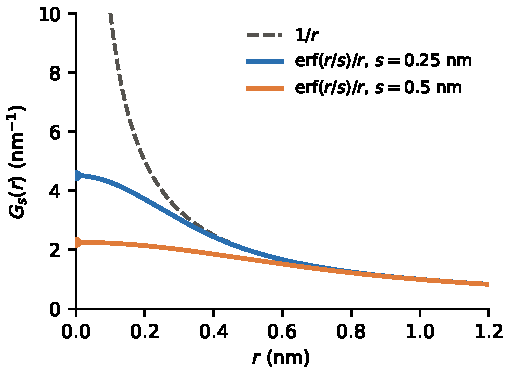
\includegraphics[width=0.5\textwidth]{fig/kernel.pdf}
  \caption{The smoothed Coulomb kernel $G_s(r) = \mathrm{erf}(r/s)/r$ against $1/r$; the dots are $G_s(0)$. The model's
  $s_e = 0.25$\,nm is the blue curve.}
  \label{fig:kernel}
\end{figure}

There are two reasons to smooth.
On a grid of spacing $\Delta x$ a cell is a blob of width $\sim\Delta x$; treating it as a Gaussian with $s=2\Delta x$
makes the grid sums smooth approximations of the integrals.
And physically, a classical Boltzmann gas collapses into a point ion ($e^{\kc q/rT}$ is not integrable at $r\to0$):
the electron's quantum size, 0.1--0.2\,nm at 10--50\,eV, blurs the singular well, and the bound part of the well is
the atomic module's.
The model uses
\begin{equation}
  s = \max\!\big(2\Delta x,\ s_e\big),\qquad s_e = \opt{mcmd-pb-smoothing} = 0.25\ \mathrm{nm},
\end{equation}
everywhere the kernel appears: the ion and electron potentials, the escape depth, distant ions and the long-range ion
force.
Once the grid resolves $s_e$ ($\Delta x\le s_e/2$), refining it no longer changes the physics.
The charge, the escape and the ion directions do not depend on $s_e$; the ion kinetic energy does
(Appendix~\ref{app:validation}).

\section{The temperature}
\label{sec:temperature}

The temperature is that of an ideal gas, $T = \frac23K/N$, with $K$ the electrons' kinetic energy --- the usual
equipartition definition, since the potential energy is explicit.
$K$ is not tracked directly: the model conserves the electrons' \emph{total} energy $E_{\mathrm{tot}} = K + U$, with
the electrostatic energy $U(\vect n) = \int n\,[-\Phi + \frac12K*n]$ (electrons with ions, and half their mutual
repulsion; the ion--ion energy is GROMACS's).
Since the density depends on $T$, $T$ and $\vect n$ are found together, from
\begin{equation}
  g(T) = E_{\mathrm{tot}} - U(\vect n_T) - \tfrac32NT = 0,
\end{equation}
where $\vect n_T$ minimizes $F$ at $T$.
A hotter cloud spreads into regions of higher potential energy, so $g$ decreases monotonically and has one root,
found by a safeguarded secant iteration (Appendix~\ref{app:numerics}).

\section{Energy bookkeeping}
\label{sec:energy}

Tracking $E_{\mathrm{tot}}$ instead of $K$ means that the adiabatic cooling of an expanding cloud, and the heating
when an ion's charge grows under it, appear by themselves in $K = E_{\mathrm{tot}} - U$.
$E_{\mathrm{tot}}$ changes only by explicit exchanges.
Write $V_e = K*n$ for the electrons' repulsion from the last solve, scaled by $\varsigma = N/N_{\mathrm{solve}}$ for
electrons added or lost since, and
\begin{equation}
  D_k = \kc\sum_{b\ne k} q_b\,G_s(|\vect x_k-\vect x_b|) - \varsigma\,V_e(\vect x_k)
  \label{eq:Dk}
\end{equation}
for the depth of the well at atom $k$: the binding energy of an electron at rest there.
\begin{enumerate}
  \item \textbf{Work on the ions.} The cloud's force on the ions does work $W$ per step, taken from the electrons:
    $\Delta E_{\mathrm{tot}} = -\sum_a\vect F_a\cdot\vect v_a\Delta t$.
  \item \textbf{A trapped photo- or Auger electron} of energy $\varepsilon$ at atom $k$:
    $\Delta E_{\mathrm{tot}} = \varepsilon - D_k$.
  \item \textbf{Collisional ionization} at $k$ with binding energy $\Delta E_{\mathrm b}$: a cloud electron pays it, and
    the freed electron starts at rest at $k$: $\Delta E_{\mathrm{tot}} = -\Delta E_{\mathrm b} - D_k$.
  \item \textbf{A change of an ion's charge} by $\Delta q$ changes its interaction with the cloud; the kinetic energy does
    not change at that instant: $\Delta E_{\mathrm{tot}} = -\Delta q\,\varsigma V_e(\vect x_k)$.
  \item \textbf{Evaporation} of $\delta N$ electrons with kinetic energy $\delta E$ from mean depth $\bar D$:
    $\Delta E_{\mathrm{tot}} = -(\delta E - \delta N\bar D)$.
  \item \textbf{A grid rebuild} changes $U$ for numerical reasons only; the change is moved into $E_{\mathrm{tot}}$ so
    that $K$ does not jump.
\end{enumerate}
An electron that escapes at birth never joins the cloud; it only raises the net charge.
\file{energy\_ledger.txt} and \file{pb\_log.txt} record these terms (Chapter~\ref{ch:output}).

\section{Forces on the ions}

An ion of charge $q_a$ has potential energy $-q_a\varsigma V_e(\vect x_a)$ in the cloud, so the cloud pulls on it with
\begin{equation}
  \vect F_a = q_a\,\varsigma\,\nabla V_e(\vect x_a),
\end{equation}
from central differences on the grid, interpolated to the atom (outside the grid: a point charge at the cloud's
centroid).
The forces are added to the GROMACS forces every step on every rank, and their work is booked (item~1).
Between solves the ions move through the fixed electron potential.

\section{Escape or trapping}
\label{sec:escape}

An electron of kinetic energy $\varepsilon$ released at atom $k$ escapes if $\varepsilon > D_k$ and is trapped
otherwise, with the depth~\eqref{eq:Dk} of the same smoothed ion potential and the same cloud the solve uses.
The atom's own new charge is left out: the electron leaves before the atom's remaining electrons rearrange.
An escaped electron adds one to the net charge $Q$; a trapped one adds one to $N$ and is booked as item~2.
Each electron is tested once, at birth: an escaped one cannot be recaptured, and a trapped one leaves only by
evaporation.

\section{Evaporation}
\label{sec:evaporation}

A well of finite depth cannot hold the tail of a Maxwell distribution: an electron whose kinetic energy exceeds its
local depth $D(\vect x) = -V(\vect x)$ is unbound and leaves, and collisions keep refilling the tail.
This evaporation (\opt{mcmd-evaporation = 1}, the default) matters late in the explosion, when the well is shallow and
the cloud still hot.
For a Maxwell distribution at $T$, the fraction of electrons above $D$ and the fraction of their kinetic energy above
$D$ are regularized incomplete gamma functions of $x = D/T$~\cite{abramowitz1964}:
\begin{equation}
  Q(\tfrac32,x) = \mathrm{erfc}\sqrt x + 2\sqrt{x/\pi}\,e^{-x},\qquad
  Q(\tfrac52,x) = Q(\tfrac32,x) + \tfrac{4}{3\sqrt\pi}x^{3/2}e^{-x}.
\end{equation}
The energy tail is the larger (Fig.~\ref{fig:tails}), so evaporation cools the cloud.
Summed over the cells of the last solve (binned by depth into 4000 bins once per solve),
$\delta N^{\mathrm{tail}} = \sum_i n_iQ(\frac32,x_i)$ and $\delta E^{\mathrm{tail}} = \frac32T\sum_in_iQ(\frac52,x_i)$.
The tail refills at the electron--electron collision rate~\cite{nrl}
\begin{equation}
  \nu_{ee} = 2.91\times10^{-6}\,n_e[\mathrm{cm^{-3}}]\,\ln\Lambda\,T^{-3/2}\ \mathrm{s^{-1}},\qquad
  \ln\Lambda = \max\big(2,\ 24-\ln(\sqrt{n_e}/T)\big),
\end{equation}
at the mean density $n_e = N/(\frac43\pi R^3)$, and every MD step a fraction $\phi = \min(1,\nu_{ee}\Delta t)$ of it
leaves: $N$ and $K$ fall by $\phi\varsigma\,\delta N^{\mathrm{tail}}$ and $\phi\varsigma\,\delta E^{\mathrm{tail}}$, the
net charge $Q$ rises, and the leavers' total energy is booked (item~5).
How many electrons evaporate depends on the box (Appendix~\ref{app:numerics}); the total that escapes, at birth and by
evaporation, does not.

\begin{figure}[t]
  \centering
  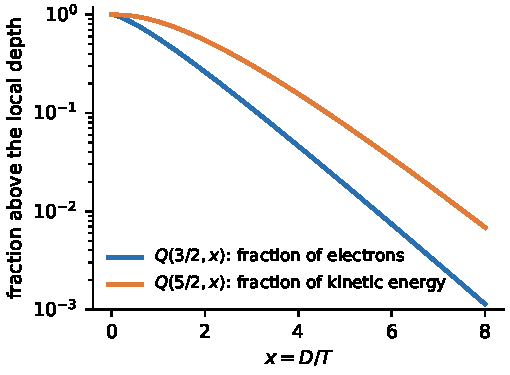
\includegraphics[width=0.5\textwidth]{fig/tails.pdf}
  \caption{The Maxwell tails above a depth $D$: the fraction of electrons $Q(\frac32,D/T)$ and of their kinetic energy
  $Q(\frac52,D/T)$.}
  \label{fig:tails}
\end{figure}

\section{Assumptions}

\begin{itemize}
  \item One temperature, instantaneous equilibrium: hot spots are averaged out at the next solve.
  \item Classical mean field: no degeneracy, exchange or correlation below the scale $s_e$; $s_e$ has a physical size
    but is not derived from first principles.
  \item Electrons frozen between solves (0.2\,fs), adequate while the ions move much less than a grid cell in that
    time.
  \item Escape at birth only; evaporation at the mean electron--electron collision rate, an estimate rather than a
    kinetic calculation.
  \item Far from the sample the cloud is a point charge.
\end{itemize}

\chapter{Electron--ion collisions and field ionization}
\label{ch:coll}

\section{Electron-impact ionization}

With the electron cloud on, its electrons ionize the atoms they reach (\opt{mcmd-collisions = 1}, the default).
Every configuration can lose one electron from each occupied shell, to any final configuration that has data.
The rate of a channel $i\to f$ at atom $k$ is
\begin{equation}
  w_{i\to f} = n_e(\vect x_k)\,\langle\sigma v\rangle_{i\to f}(T),
\end{equation}
with the cloud's temperature $T$ and its density at the atom, interpolated from the last solve,
$n_e(\vect x_k) = \varsigma\sum_{\vect o}w_{\vect o}\,n_{\vect i_0+\vect o}/\Delta V$ (cloud-in-cell weights).
An ion deep in the quasi-neutral core sees a high density and ionizes quickly; one in the depleted outer sheath sees
almost none.
The collisional channels join the atom's other transitions in the Monte Carlo step, with the rates frozen for the
step, and the energy is booked as in Section~\ref{sec:energy} (item~3).
The transition energy is always $\Delta E = T_i - T_f$ from the total energies.

\subsection{Rate coefficients: Lotz (built in) or from files}

\opt{mcmd-coll-data} chooses where $\langle\sigma v\rangle$ comes from.
\begin{description}
  \item[\code{lotz}] (default): Lotz's Maxwellian formula~\cite{lotz1968} (with $b=0$),
    \begin{equation}
      \langle\sigma v\rangle = 6.7\times10^{-7}\,a\,q\,T^{-3/2}\,\frac{E_1(P/T)}{P/T}\ \ \mathrm{cm^3\,s^{-1}},\qquad
      a = 4.5\times10^{-14}\ \mathrm{cm^2\,eV^2},
    \end{equation}
    $q$ the occupation of the shell, $P = \Delta E$ (eV), $E_1$ the exponential integral.
    No data file is needed.
  \item[\code{files}]: from \file{collisional\_ionization\_table\_X.txt} if present, a table of
    $\langle\sigma v\rangle$ on a temperature grid that any atomic code can supply; else from the Sampson fits in
    \file{collisional\_parameters\_X.txt} (CRETIN models):
    \begin{equation}
      \langle\sigma v\rangle = 1.0899\times10^{-6}\,\frac{s_0\,q(b)}{\Delta E\sqrt T}\,e^{-b},\quad
      q(b) = c_0 + c_1\sqrt{\pi b}\,\mathrm{erfcx}\sqrt b + (c_2b+c_3)\,e^bE_1(b),\quad b = \frac{\Delta E}{T}.
    \end{equation}
    Tables are interpolated linearly in $\ln T$ in the smooth quantity $\ln\langle\sigma v\rangle + \Delta E/T$ and
    held at the grid edges outside them.
\end{description}
For H, C, N, O and S Lotz gives the same transitions as the CRETIN fits, with coefficients 13--25\,\% higher
between 10 and 300\,eV.
On lysozyme at 600\,eV this changes the ion kinetic energy by $-2.5$\,\% and nothing else beyond the seed noise.
A \file{.tpr} older than format 79 runs as \code{files}.

\section{Three-body recombination}

The inverse of collisional ionization, two cloud electrons colliding at an ion with one of them captured, follows by
detailed balance with the statistical weights $g$:
\begin{equation}
  w_{f\to i} = n_e^2\,\langle\sigma v\rangle_{i\to f}\,\frac{g_i}{g_f}\,1.656\times10^{-22}\,T^{-3/2}\ \ \mathrm{s^{-1}}.
\end{equation}
It is off by default (\opt{mcmd-coll-recombination = 0}) and \textbf{not fully validated}: in the classical
continuum picture it recaptures far too many electrons in the dense, cool cloud late in the explosion.
\opt{mcmd-coll-h-recombination} additionally allows recombination onto hydrogen (off: a proton stays a proton).

\section{Collisional excitation}

With \opt{mcmd-coll-excitation = 1} the cloud also excites atoms between configurations with the same number of
electrons, and de-excites them by detailed balance ($\langle\sigma v\rangle_{\mathrm{down}} =
\langle\sigma v\rangle_{\mathrm{up}}\,g_{\mathrm{lower}}/g_{\mathrm{upper}}$).
The rates come from \file{collisional\_excitation\_table\_X.txt} or the CRETIN \code{colex2} fits in
\file{collisional\_excitation\_X.txt} (Chapter~\ref{ch:data}).
It is off by default and \textbf{not fully validated}: it produces too much early collisional ionization out of excited
configurations.

\section{Field ionization}

In a strongly charged sample the collective field can lower an atom's barrier below its outermost binding energy.
With \opt{mcmd-field-ionization = 1} an atom is stripped while the field at it exceeds the Bethe over-the-barrier
threshold,
\begin{equation}
  F \ge \frac{I_p^2}{4\kc Z},
\end{equation}
$I_p$ the binding energy of its outermost electron and $Z$ its charge after the step.
$F = |\nabla P_L|$ is the field of the collective potential $P_L = \kc G_L*(q_{\mathrm{ion}}-n_e)$, with every
charge spread over $L$ (\opt{mcmd-field-ionization-smoothing}, 0.5\,nm; at least the grid's $s$) and the atom's own
charge left out, so neighbours closer than $\sim L$ are smeared: their barrier lowering is the charge-transfer
channel's.
It is computed on the grid after every solve, by direct summation where there is no grid, during the pulse only
(from 6$\sigma_t$ before to 4$\sigma_t$ after the peak, stopping once no atom has been within a factor 2 of its
threshold for 5 updates).
Every field ionization is logged in \file{pbfield\_events.txt}.

Field ionization does not change the explosion: on ubiquitin at 600\,eV it strips $\sim$900--1000 atoms per run early in
the pulse, and about as many fewer are ionized by electron impact and charge transfer; the charge, the escape and the
ion directions are unchanged.
It is off by default.

\chapter{Atomic data}
\label{ch:data}

By default the module computes the atomic physics of every element at start-up from a screened-hydrogenic shell
model, for the photon energy of the pulse (\opt{mcmd-atomic-data = hydrogenic}, Section~\ref{sec:builtin}); no input
file is needed.
With \opt{mcmd-atomic-data = files} it reads the same quantities from plain-text tables in \file{./Atomic\_data/} of
the run directory instead.
This chapter specifies the tables; \file{ATOMIC\_DATA.md} in the repository is the same specification in short form,
and \file{tools/check\_atomic\_data.py} checks a directory against it.

\section{The built-in data}
\label{sec:builtin}

The built-in data are a screened-hydrogenic model of shells only~\cite{scott2010}, with the screening constants of
Marchand, Caille and Lee~\cite{marchand1990} and the level energies scaled to the NIST ionization
energies~\cite{nist}:
\begin{itemize}
  \item states: every \code{K L M} of every charge state ($K \le 2$, $L \le 8$, $M \le 18$), so elements up to
    $Z = 18$ (H to Ar except He); Ca, Fe, Ni and I need \opt{mcmd-atomic-data = files};
  \item energies: the screened-hydrogenic binding energy of each configuration (with the leading relativistic
    terms), the excitation energy scaled by the ratio of the NIST to the hydrogenic ionization energy of the charge
    state its lowest inner-shell hole belongs to;
  \item photoionization out of each occupied shell: Kramers' cross section with a constant Gaunt factor,
    $\sigma \propto q^4 n^{-5} E^{-3}$ per electron ($q$ the screened charge of the shell);
  \item fluorescence: the Einstein $A$ of each radiative transition into a lower shell, from hydrogenic oscillator
    strengths scaled with the screened charges;
  \item Auger: the hydrogenic formula of Scott and Hansen~\cite{scott2010} (Gaunt factor 0.12), summed per final state;
  \item statistical weights $g = \binom{2}{K}\binom{8}{L}\binom{18}{M}$.
\end{itemize}
It takes well under a second.
The model is the one of the CRETIN screened-hydrogenic models the published results were computed with; it reproduces
their rates to $\sim$10\,\% and, on lysozyme at 1000\,eV, their explosion: charge to 0.7\,\%, escape to 1.3\,\%,
directions within the seed noise, ion kinetic energy 3.5\,\% lower (Section~\ref{sec:accuracy}).
There are no collisional fit data: electron-impact ionization comes from Lotz's formula (\opt{mcmd-coll-data = lotz}),
and collisional excitation (\opt{mcmd-coll-excitation}) and \opt{mcmd-coll-data = files} need
\opt{mcmd-atomic-data = files}; \code{grompp} stops otherwise.
The run writes the data it used to \file{simulation\_output/Atomic\_data/}, in the format below; copied to
\file{./Atomic\_data} and run with \opt{mcmd-atomic-data = files} they give the identical run.

\section{Which files}

A file is \file{<table>\_<SYMBOL>.txt}, with the symbol in upper case as in Table~\ref{tab:elements}
(\file{energy\_levels\_C.txt}, \file{rate\_transitions\_CL.txt}).
Only the elements present in the system are needed.

\begin{table}[H]
\centering\small
\begin{tabularx}{\textwidth}{@{}>{\raggedright\arraybackslash}p{0.4\textwidth} X X@{}}
\toprule
file & needed when (\opt{mcmd-atomic-data = files}) & what for \\
\midrule
\file{energy\_levels\_X.txt} & always & outermost binding energy per state \\
\file{rate\_transitions\_X.txt} & always & photoionization, Auger, fluorescence \\
\file{total\_energies\_X.txt} & charge transfer or collisions on (both default) & electron energies, charge-transfer
  energies, collisional transition energies \\
\file{statistical\_weight\_X.txt} & collisions on & detailed balance \\
\file{collisional\_ionization\_table\_X.txt} or \file{collisional\_parameters\_X.txt} &
  only with \opt{mcmd-coll-data = files} & electron-impact ionization \\
\file{collisional\_excitation\_table\_X.txt} or \file{collisional\_excitation\_X.txt} &
  only with \opt{mcmd-coll-excitation = 1} & collisional (de-)excitation \\
\bottomrule
\end{tabularx}
\end{table}
Only \file{rate\_transitions\_X.txt} depends on the photon energy (the photoionization cross sections): regenerate it
for every \opt{mcmd-pulse-photon-energy}.

\paragraph{General rules.}
One record per line, whitespace separated; \code{;} separates the initial state from the final states in the
transition tables; no comments or header (except the tables' temperature line).
Lines must be shorter than 1024 characters.
Energies in eV, rates in s$^{-1}$, cross sections in cm$^2$.
Where a state appears twice, the first line counts.

\section{The tables}

\paragraph{\file{energy\_levels\_X.txt}:} \code{K L M E}, the binding energy of the state's \emph{outermost}
electron.
Autoionizing states (excitation above the ionization potential of their charge state) get \code{1e14}.
Used as the charge-transfer donor energy and the field-ionization threshold.

\paragraph{\file{total\_energies\_X.txt}:} \code{K L M T}, the energy to remove all of the state's electrons,
$T = \sum(\text{ionization potentials up to this charge state}) - \text{excitation energy}$; defined for autoionizing
states too, and \code{0 0 0 0.0}.
It must reproduce \file{energy\_levels} for every bound state, $E(c) = T(c) - T(c\text{ minus its outermost
electron})$, and cover every reachable state.
It gives the kinetic energy of emitted electrons (photoelectron $E_{\mathrm{ph}} - (T_{\mathrm{from}}-T_{\mathrm{to}})$,
Auger $T_{\mathrm{to}} - T_{\mathrm{from}}$, both must be positive), the binding energy of any shell for charge
transfer, and collisional transition energies.

\paragraph{\file{rate\_transitions\_X.txt}:} one line per initial state, then one \code{;}-terminated token per final
state with five fields:
\begin{lstlisting}
K L M ;K' L' M' rate type ;K'' L'' M'' rate type ;...
1 1 0 ;1 0 0 7.416614e-21 2 ;0 1 0 0.0 2 ;2 0 0 7.291753e+11 1 ;      (oxygen, 600 eV)
\end{lstlisting}
Type 0: Auger--Meitner decay, rate in s$^{-1}$, one electron fewer.
Type 1: fluorescence, rate in s$^{-1}$, same electron count.
Type 2: photoionization, cross section in cm$^2$, one electron fewer.
The type column is mandatory: many Auger and photoionization transitions have the same occupation change.
Every state reachable through any transition needs a line of its own, also without transitions (\code{K L M ;});
only \code{0 0 0} may be absent.
A zero rate is inactive; two entries to the same final state are two channels.

\paragraph{\file{statistical\_weight\_X.txt}:} \code{K L M g}, the degeneracy $g = \binom{2}{K}\binom{8}{L}\binom{18}{M}$.

\paragraph{Collisional data} (only for \opt{mcmd-coll-data = files} and collisional excitation):
\begin{itemize}
  \item \file{collisional\_ionization\_table\_X.txt}, \file{collisional\_excitation\_table\_X.txt}: a first line
    \code{T\_e t1 ... tn} (eV, increasing, full precision), then \code{K L M K' L' M' k1 ... kn}: the full Maxwellian
    rate coefficient $\langle\sigma v\rangle$ (cm$^3$\,s$^{-1}$, Boltzmann factor included) at each temperature.
    Any exponent is allowed (\code{3.1e-2650}); a \code{0} means too small to write and is extrapolated.
    The tables are generator independent: FLYCHK, FAC, BEB or Lotz can supply them.
  \item \file{collisional\_parameters\_X.txt} (\code{K L M ; K' L' M' c0 c1 c2 c3 s0 ; ...}) and
    \file{collisional\_excitation\_X.txt} (\code{... c0 c1 c2 c3 a0 ...}): the CRETIN Sampson and \code{colex2} fits,
    used where no table is given (formulas in Chapter~\ref{ch:coll}).
\end{itemize}

\section{Generating the data}
\label{sec:generators}

Two generators write all the tables above, for \opt{mcmd-atomic-data = files}.

\paragraph{From XATOM} (\file{tools/make\_atomic\_data\_xatom.py OUTDIR ENERGY [--elements H,C,N,O,S] [--validate]}).
XATOM~\cite{jurek2016,son2011} is an open-source (GPLv3) Hartree--Fock--Slater atomic code; its output is not covered
by its license, so the generated data can be distributed freely.
The script runs \code{xatom} once per configuration ($\sim$20\,s for H, C, N, O, S on 12 cores):
\begin{itemize}
  \item states: every \code{K L M} up to the ground-state occupation --- photoionization, Auger, fluorescence and charge
    transfer never leave that set;
  \item each state is computed as its aufbau subshell configuration (2s before 2p, 3s before 3p), and XATOM's subshell
    final states are summed back onto \code{K L M};
  \item energies from the orbital eigenvalues,
    $T(c) = T(c\text{ minus its outermost electron}) - \varepsilon_{\mathrm{outermost}}(c)$: XATOM's total energies are
    tens of eV off (N$^{5+}$\,1s$^2$: 1267\,eV against 1218), its eigenvalues are what it prices transitions with;
  \item core and valence photoionization (\code{P}, \code{V}) become type 2, \code{A} type 0, \code{F} type 1;
    photoexcitation is dropped; channels these energies close and intra-shell ones are dropped and counted;
  \item elements up to $Z = 18$ (H to Ar except He); Ca, Fe, Ni are refused (their 4s electrons are
    counted in M).
\end{itemize}

\paragraph{From CRETIN models} (\file{tools/make\_atomic\_data\_cretin.py MODELS OUTDIR ENERGY [--tables] [--validate]}).
Reads CRETIN \file{.z01} atomic models and writes all tables including the Sampson and \code{colex2} fits;
\code{--tables} also writes them as temperature tables (\file{tools/make\_collisional\_tables.py}).
CRETIN is not open source.

\paragraph{Checking.}
\code{tools/check\_atomic\_data.py Atomic\_data --photon-energy E} reports everything the reader would stop on or
misread as an error and everything legal but suspicious (rates out of range, closed channels, unreachable states) as a
warning; it exits 1 on errors.

\section{Accuracy of the data}
\label{sec:accuracy}

Against Scofield's subshell photoionization cross sections~\cite{scofield1973} and Krause's K-shell widths and
fluorescence yields~\cite{krause1979} (via xraylib):
\begin{table}[H]
\centering\small
\begin{tabular}{lccc}
\toprule
ground state, 600\,eV, kb & Scofield & XATOM & CRETIN \\
\midrule
C K / L & 167.8 / 7.86 & 167.8 / 7.86 & 179.5 / 1.61 \\
N K / L & 275.9 / 14.4 & 276.0 / 14.4 & 317.6 / 4.13 \\
O K / L & 411.3 / 24.5 & 411.5 / 24.5 & 507.9 / 9.05 \\
S L / M & 445.9 / 26.6 & 444.7 / 26.5 & 419.2 / 2.19 \\
\bottomrule
\end{tabular}
\end{table}
XATOM agrees with Scofield to 0.3\,\% and with Krause for the S K hole (width 0.56 against 0.52\,eV, fluorescence yield
0.089 against 0.080).
The CRETIN models' K-shell cross sections are 7--23\,\% high, their valence ones 3--12$\times$ low, and their S K-hole
Auger rate 3.4$\times$ low.
XATOM's weak point is the outermost binding energy of neutral C and N ($\sim$20\,\% low, open 2p shells).
On lysozyme at 600\,eV, XATOM data give a 15\,\% higher ion kinetic energy than CRETIN data, 1\,\% more charge, and the
same ion directions; at 1000\,eV (the example) 39\,\% higher, with half the Auger decays and twice the valence
photoionizations.

The built-in data are of the CRETIN kind: core photoionization within 10\,\% of the CRETIN models, valence within
5\,\%, Auger and fluorescence per configuration within $\sim$10\,\%, so with the same deviations from the reference
data; their K-hole Auger rates are 1.5--2.5$\times$ slower than CRETIN's, and the constant Gaunt factor makes the
photoionization rise above CRETIN's towards 10\,keV (C, N, O core 1.3$\times$ at 12\,keV).

\chapter{Output}
\label{ch:output}

All standard GROMACS output (\file{.trr}, \file{.edr}, \file{.log}, \file{.gro}) is written as usual.
The ionization module writes into \file{simulation\_output/} in the run directory; a 30\,fs lysozyme run writes about
0.6\,MB there.
Text files are whitespace-separated columns (\code{numpy.loadtxt} reads them; \code{\#} lines are headers); times are in
ps.
The time-resolved files are written every \code{nstenergy} steps, the electron model's at every solve; all are
buffered and flushed every 1000 steps.

\section{Always written}

\begin{description}
  \item[\file{charges.txt}] the final charge of every atom: atom number (1-based), charge.
  \item[\file{procces\_statistics.txt}] event counts at the end: Auger decays, fluorescence, photoionizations, charge
    transfers.
    (Electron-impact ionizations and recombinations are in \file{collisional\_log.txt} and in the end-of-run summary
    on stderr.)
  \item[\file{masses.bin}] the atom masses (float32), from which \file{tools/mcmd\_output.py} gets the elements.
  \item[\file{mcionize\_state.bin}] the restart state, written at every checkpoint (Section~\ref{sec:seed}); the
    previous one is kept as \file{mcionize\_state\_prev.bin}.
  \item[\file{timing\_mcionize.txt}] wall time per part of the module (Monte Carlo, charge transfer, PB solves, \ldots).
\end{description}

\section{Time-resolved output (\opt{mcmd-detailed-output = 1})}

\begin{description}
  \item[\file{mean\_charge\_vs\_time.txt}] $t$, mean charge per atom.
  \item[\file{pulse\_profile.txt}] $t$, pulse intensity $I(t)$ in photons\,cm$^{-2}$\,s$^{-1}$.
  \item[\file{electron\_data.txt}] $t$, mean density of the trapped electrons (cm$^{-3}$), their temperature (eV), and
    the expansion $R_g/R_g(0)$.
    The temperature is \code{nan} before the first electron is trapped.
  \item[\file{charges\_over\_time.bin}] every atom's charge (float32), one frame every
    \opt{mcmd-charge-output-stride} steps (default 500, i.e.\ 1\,fs at 2\,as).
  \item[\file{transitions.bin}] every electronic event: a 16-byte header (\code{MCMDTRN1}, version, record size), then
    20-byte records: time (fs, float32), atom (0-based), the charge-transfer donor (else $-1$), the type (0 Auger,
    1 fluorescence, 2 photoionization, 3 collisional ionization, 4 recombination, 5 excitation, 6 de-excitation,
    7 charge transfer), and the \code{K L M} occupations before and after.
    It is front-loaded: photoionization follows the pulse and the Auger cascades follow within a few fs.
\end{description}

\section{The electron model (\opt{mcmd-electrons = pbgrid})}

\begin{description}
  \item[\file{pb\_log.txt}] one line per solve: $t$, $N$ trapped, $Q$ escaped, $T$, grid spacing, ions outside the
    grid, Newton and CG iterations, residual, wall time (ms), mean and maximum depth, the field's work and the change of
    $U$ since the last solve, the kinetic energy, any clamped energy, the core neutralization (electrons per ion charge
    within $R/2$), convolutions, rebuilds, temperature iterations.
  \item[\file{screening\_log.txt}] every \code{nstenergy} steps: escaped and trapped electrons, trapped fraction, mean
    energy of the trapped electrons, $R$, Debye length and number, evaporated electrons, $T$.
  \item[\file{collisional\_log.txt}] every \code{nstenergy} steps: $T$, mean $n_e$, $N$, the cloud's energy, cumulative
    electron-impact ionizations and recombinations, the energy spent on ionization, the energy brought in by trapped
    electrons, the adiabatic and evaporated energy, $R$, $Q$.
    It is written before each step's Monte Carlo, so the last line misses the last step's events; the end-of-run
    summary has the final counts.
  \item[\file{energy\_ledger.txt}] cumulative energy exchanges: the ion--ion and ion--electron energy jumps of charge
    changes, the field's work on the ions, the electrons' kinetic energy, $N$.
  \item[\file{pbg\_box.txt}] the grid box at each solve: $R$, half-width in units of $R$, spacing, the estimated fraction
    of electrons outside, whether the grid was rebuilt, cells per side.
  \item[\file{pbg\_lr.txt}] with long range: the refreshes of the long-range ion field.
  \item[\file{pbfield\_events.txt}] with field ionization: every event ($t$, atom, mass, charge after, distance from
    the centre, field, $I_p$, depth).
\end{description}

\section{The output viewer}
\label{sec:viewer}

\file{tools/mcmd\_output.py} reads all of the above:
\begin{lstlisting}
mcmd_output.py transitions [dir] [--type photo,auger] [--atom 12] [--tmin 20 --tmax 40]
mcmd_output.py summary [dir]           # events per type and element, and per 5 fs
mcmd_output.py charges [dir]           # mean charge per element over time
mcmd_output.py plot [dir]              # overview.png of every metric the run wrote
mcmd_output.py plot [dir] --gif        # + explosion.gif: three views along the initial gyration axes
mcmd_output.py plot [dir] --extract    # + extracted/: transitions.txt, charges_over_time.txt
\end{lstlisting}
\code{dir} is the run directory or its \file{simulation\_output} (default: the current directory).
From Python, \code{import mcmd\_output} gives \code{read\_transitions}, \code{read\_charges}, \code{elements},
\code{masses} and \code{read\_trr} (pure Python) as numpy arrays.

\chapter{Reference: mdp options}
\label{ch:mdp}

All options of the model are \code{mcmd-*} entries in the \file{.mdp} file.
They take effect only with \code{mdrun -ionize}; without it the run is stock GROMACS~4.5.4 whatever the \file{.mdp}
says.
\code{grompp} rejects unknown \code{mcmd-*} keys and the removed ones, with the replacement.
The defaults are the validated model; settings marked ``not fully validated'' are listed by
the run summary as warnings (Section~\ref{sec:summary}).
Times of the pulse and of the electron model are in \textbf{fs}, unlike \code{dt} and \code{tinit}.

\newcommand{\optrow}[4]{\code{#1} & #2 & #3 & #4 \\}

\section{The pulse}
\begin{longtable}{@{}p{0.36\textwidth} p{0.09\textwidth} p{0.07\textwidth} >{\raggedright\arraybackslash}p{0.4\textwidth}@{}}
\toprule
option & default & unit & meaning \\ \midrule \endhead
\optrow{mcmd-pulse-peak-time}{0}{fs}{centre of the Gaussian pulse}
\optrow{mcmd-pulse-fwhm}{0}{fs}{full width at half maximum}
\optrow{mcmd-pulse-photons}{0}{}{photons in the pulse; 0: no ionization (warning)}
\optrow{mcmd-pulse-focal-diameter}{0}{nm}{diameter of the focal spot, uniform over the sample}
\optrow{mcmd-pulse-photon-energy}{0}{eV}{photon energy; the built-in data are computed for it, files must be
  generated for it}
\optrow{mcmd-pulse-bandwidth}{0.003}{}{relative FWHM of the photon energy: jitters the photoelectron energies}
\bottomrule
\end{longtable}

\section{Atomic data}
\begin{longtable}{@{}p{0.35\textwidth} p{0.12\textwidth} p{0.05\textwidth} >{\raggedright\arraybackslash}p{0.4\textwidth}@{}}
\toprule
option & default & unit & meaning \\ \midrule \endhead
\optrow{mcmd-atomic-data}{hydrogenic}{}{\code{hydrogenic}: built in, screened-hydrogenic shells, H to Ar except He, no input
  file (Section~\ref{sec:builtin}); \code{files}: the tables in \file{./Atomic\_data}}
\bottomrule
\end{longtable}

\section{Charge transfer}
\begin{longtable}{@{}p{0.36\textwidth} p{0.09\textwidth} p{0.07\textwidth} >{\raggedright\arraybackslash}p{0.4\textwidth}@{}}
\toprule
option & default & unit & meaning \\ \midrule \endhead
\optrow{mcmd-charge-transfer}{1}{}{over-the-barrier charge transfer (Chapter~\ref{ch:ct})}
\optrow{mcmd-ct-h-donor-only}{1}{}{only neutral hydrogen donates (the published model); 0 is not fully validated}
\optrow{mcmd-allow-h-ct}{0}{}{allow H--H transfer (resonant); not fully validated}
\optrow{mcmd-charge-transfer-downhill}{0}{}{require the transfer to be downhill, Coulomb release included}
\optrow{mcmd-charge-transfer-idle}{2000}{steps}{steps without a transfer before the pass goes idle; negative: never}
\optrow{mcmd-charge-transfer-recheck}{100}{steps}{interval of the idle pass}
\bottomrule
\end{longtable}

\section{The electron cloud}
\begin{longtable}{@{}p{0.36\textwidth} p{0.09\textwidth} p{0.07\textwidth} >{\raggedright\arraybackslash}p{0.4\textwidth}@{}}
\toprule
option & default & unit & meaning \\ \midrule \endhead
\optrow{mcmd-electrons}{pbgrid}{}{\code{pbgrid}: the Poisson--Boltzmann cloud (Chapter~\ref{ch:pb}); \code{none}:
  every electron leaves}
\optrow{mcmd-pb-smoothing}{0.25}{nm}{the electron size $s_e$; the ion kinetic energy depends on it (warning if
  changed)}
\optrow{mcmd-pb-interval}{0.2}{fs}{time between PB solves (and long-range refreshes); converged at 0.2}
\optrow{mcmd-pb-newton-tol}{0.01}{}{Newton stop: relative residual; converged at 0.01}
\optrow{mcmd-pb-cells-per-smoothing}{2.5}{}{target spacing $s_e/$this at the start; converged at 2.5}
\optrow{mcmd-pb-box-cut}{0.02}{}{the box grows when more than this fraction of the electrons would be outside;
  0: fixed box of \code{mcmd-pb-box-max}}
\optrow{mcmd-pb-box-max}{3}{$R$}{largest box half-width}
\optrow{mcmd-pb-grid-limit}{384}{cells}{most cells per side; a warning in \file{md.log} says when a sample needs more}
\optrow{mcmd-pb-long-range}{auto}{}{\code{auto}: above 10\,000 atoms a 2\,nm cutoff plus the long-range ion force
  from the grid, else all pairs (\code{grompp} sets the cut-offs); \code{1}/\code{0} keep the mdp's cut-offs}
\optrow{mcmd-evaporation}{1}{}{evaporation of the cloud; 0 is not fully validated}
\bottomrule
\end{longtable}

\section{Collisions and field ionization}
\begin{longtable}{@{}p{0.36\textwidth} p{0.09\textwidth} p{0.07\textwidth} >{\raggedright\arraybackslash}p{0.4\textwidth}@{}}
\toprule
option & default & unit & meaning \\ \midrule \endhead
\optrow{mcmd-collisions}{1}{}{electron-impact ionization in the cloud (Chapter~\ref{ch:coll})}
\optrow{mcmd-coll-data}{lotz}{}{\code{lotz}: built-in formula; \code{files}: tables or fits from \file{Atomic\_data}}
\optrow{mcmd-coll-recombination}{0}{}{three-body recombination; not fully validated}
\optrow{mcmd-coll-h-recombination}{0}{}{recombination also onto hydrogen}
\optrow{mcmd-coll-excitation}{0}{}{collisional excitation and de-excitation; not fully validated}
\optrow{mcmd-field-ionization}{0}{}{over-the-barrier ionization in the cloud's field}
\optrow{mcmd-field-ionization-smoothing}{0.5}{nm}{$L$ of the collective field}
\bottomrule
\end{longtable}
\code{mcmd-collisions}, \code{mcmd-field-ionization} and \code{mcmd-pb-long-range = 1} need the cloud, and
\code{mcmd-coll-data = files} and \code{mcmd-coll-excitation = 1} need \code{mcmd-atomic-data = files}; \code{grompp}
stops otherwise.

\section{Run control and output}
\begin{longtable}{@{}p{0.36\textwidth} p{0.09\textwidth} p{0.07\textwidth} >{\raggedright\arraybackslash}p{0.4\textwidth}@{}}
\toprule
option & default & unit & meaning \\ \midrule \endhead
\optrow{mcmd-seed}{$-1$}{}{random seed; $-1$: new each run, printed in the summary}
\optrow{mcmd-detailed-output}{1}{}{the time-resolved output (Chapter~\ref{ch:output})}
\optrow{mcmd-charge-output-stride}{500}{steps}{frames of \file{charges\_over\_time.bin}}
\optrow{mcmd-autostop}{0}{}{stop once the kinetic energy exceeds a fraction of the total}
\optrow{mcmd-autostop-threshold}{0.99}{}{that fraction}
\optrow{mcmd-initial-charges}{0}{}{read starting charges from \file{charges.txt} (atom, charge)}
\bottomrule
\end{longtable}

\section{GROMACS settings for an explosion run}
\begin{itemize}
  \item \code{dt = 0.000002} (2\,as): the model is converged at $\le$2\,as (warning above);
  \item \code{morse = yes}: bonds that can break (Chapter~\ref{ch:ff});
  \item \code{pbc = no}, \code{coulombtype = Cut-off}, no temperature or pressure coupling;
  \item cut-offs: left to \code{mcmd-pb-long-range = auto};
  \item \code{nstenergy}: the interval of the module's time-resolved text output.
\end{itemize}

\section{Renamed and removed options}

Earlier versions used GROMACS's generic \code{userint}/\code{userreal} slots; \code{grompp} rejects them and names
the replacement:
\begin{table}[H]
\centering\small
\begin{tabular}{@{}ll@{}}
\toprule
old & new \\ \midrule
\code{userint1} & removed: \code{-ionize} alone enables the modified force field \\
\code{userint2} & \code{mcmd-charge-transfer} \\
\code{userint3} & \code{mcmd-autostop} \\
\code{userint4} & removed: use \code{mdrun -cpi} \\
\code{userint5} & \code{mcmd-detailed-output} \\
\code{userint6} & removed (never implemented): electron-impact ionization is \code{mcmd-collisions} \\
\code{userint7}, \code{userint8} & \code{mcmd-charge-transfer-idle}, \code{-recheck} \\
\code{userint9} & \code{mcmd-initial-charges} \\
\code{userreal1} & \code{mcmd-pulse-peak-time}, now in fs (multiply by 1000) \\
\code{userreal2} & \code{mcmd-pulse-photons} \\
\code{userreal3} & \code{mcmd-pulse-fwhm}, now the FWHM in fs (multiply by 2354.82) \\
\code{userreal4}, \code{userreal5} & \code{mcmd-pulse-focal-diameter}, \code{-photon-energy} \\
\code{userreal6} & \code{mcmd-autostop-threshold} \\
\bottomrule
\end{tabular}
\end{table}
The development versions of the electron model were controlled by \code{GMX\_MCMD\_*} environment variables.
Those that became options (\code{GMX\_MCMD\_SCREEN}, \code{\_SEED}, \code{\_PB\_NSTEP}, \code{\_PBG\_SE}, \ldots) and those
that were removed stop \code{mdrun} with a message naming the replacement, so an old launcher cannot run a different
model unnoticed.

\chapter{Reference: diagnostic environment variables}
\label{ch:env}

The model itself is set entirely in the \file{.mdp}.
A few environment variables remain, for diagnostics only: they add output or checks, and the physics is the same with
or without them (except for the thread count of the FFTs, which can change the last bits of the solve).
Set them to 1 to switch them on.

\begin{longtable}{@{}p{0.3\textwidth} p{0.66\textwidth}@{}}
\toprule
variable & effect \\ \midrule \endhead
\env{GMX\_MCMD\_TIMING\_DETAIL} & \file{pbg\_timing.txt}: per solve, the Newton and CG iterations, convolutions, and
  the time in FFTs, convolutions, CG and Newton; the residuals. Small overhead. \\
\env{GMX\_MCMD\_PB\_EDIAG} & \file{pb\_ediag.txt}: per solve, the split of the electrons' energy (kinetic, electron--ion,
  electron--electron, the exchanges since the last solve), for checking the energy bookkeeping. \\
\env{GMX\_MCMD\_PBG\_DENSITY} & \file{pbg\_density.bin}: the grid density every tenth solve (header $t$, $N$, $T$,
  $\Delta x$, origin, $n_g$, then $n_g^3$ floats in nm$^{-3}$). Large: hundreds of MB to GB per run. \\
\env{GMX\_MCMD\_COLL\_EVLOG} & \file{coll\_event\_log.txt}: every collisional event with the local density and
  temperature. Large. \\
\env{GMX\_MCMD\_PBG\_OUTLAT\_CHECK} & compares the sub-lattice potential of the ions outside the box with the exact sum
  (\file{pbg\_outlat.txt}) and logs the ions and time per stride level (\file{pbg\_outpot.txt}). Slow. \\
\env{GMX\_MCMD\_PBG\_LR\_CHECK} & with long range: compares the grid's long-range ion field with the exact all-pairs
  field at every refresh (\file{pbg\_lr.txt}). $O(N^2)$ on the master. \\
\env{GMX\_MCMD\_PD\_CHECK} & under particle decomposition: every 50 steps, checks each rank's coordinates against the
  master's copy (the master needs all coordinates for the solve). \\
\env{GMX\_MCMD\_PBG\_FFT\_THREADS} & threads for the FFTs of the solve; default the number of ranks
  (Appendix~\ref{app:parallel}). \\
\bottomrule
\end{longtable}

Every \code{GMX\_MCMD\_*} variable of the development versions that is not in this table is refused: \code{mdrun}
stops and names the mdp option that replaced it, or says that it was removed.


\appendix
\chapter{Numerics of the electron model}
\label{app:numerics}

This appendix describes how the free energy of Chapter~\ref{ch:pb} is discretized and minimized, and the devices that
keep the solve affordable for $10^3$--$10^5$ atoms: an adaptive grid, an adaptive box, sub-lattices for distant ions,
and the long-range ion force from the grid.
The code is in \file{src/kernel/mcionize.c}.

\section{The grid}

The grid is a cube of $n_g^3$ nodes with spacing $\Delta x$ and half-width $h$, centred on the heavy-atom centre of
mass $\vect c$: $\vect x_{ijk} = \vect c - h(1,1,1) + \Delta x\,(i,j,k)$, $\Delta x = 2h/(n_g-1)$.
The variables are the electron counts $n_i$ at the nodes, $\sum_in_i = N$, the density $n_i/\Delta V$.
The sample radius $R = (a_1a_2a_3)^{1/3}$ is that of the heavy-atom, mass-weighted gyration ellipsoid
($a_\alpha = \sqrt{5\lambda_\alpha}$), the radius of a uniform sphere; hydrogens are left out because the fast protons
leave the cloud behind.

Each charged atom inside the grid is deposited onto its 8 surrounding nodes with cloud-in-cell (trilinear)
weights~\cite{birdsall1991,hockney1988}; the same weights interpolate grid quantities back to an atom.
With $K_{ij} = \kc G_s(|\vect x_i-\vect x_j|)$ and $\Phi_i$ the ions' potential at node $i$, the discrete free energy,
its gradient and Hessian are
\begin{gather}
  F(\vect n) = \sum_i n_i\Big[-\Phi_i + \tfrac12(\Kmat\vect n)_i + T\Big(\ln\frac{n_i}{\Delta V}-1\Big)\Big],\\
  g_i = V_i + T\ln\frac{n_i}{\Delta V},\quad V_i = -\Phi_i + (\Kmat\vect n)_i,\qquad H_{ij} = K_{ij} + \frac{T}{n_i}\delta_{ij}.
\end{gather}
At the minimum on $\sum n_i = N$ all $g_i$ are equal to $\mu$.

\section{Open-boundary convolution by FFT}

Every product $\Kmat\vect a$ is a discrete convolution, and the dominant cost.
A periodic FFT of size $n_g^3$ would add the images of neighbouring boxes; the \emph{aperiodic} convolution is computed
exactly by Hockney's method~\cite{hockney1970,eastwood1979}: embed $\vect a$ in a zero-padded grid of $(2n_g)^3$,
tabulate the kernel on the same doubled grid at the minimum-image separation, multiply the transforms and transform
back.
No two physical nodes are more than $n_g-1$ apart, so the circular convolution on the doubled grid is the aperiodic one.
The kernel transform depends only on $\Delta x$ and $s$ and is computed once per grid rebuild.
FFTW~\cite{frigo2005} in single precision, real-to-complex, multithreaded; one convolution costs two FFTs of size
$(2n_g)^3$.

\section{Newton's method}

The minimizer is found by Newton's method on the constraint surface~\cite{nocedal2006}: the step $\vect d$ minimizes
$\vect g^{\mathsf T}\vect d + \frac12\vect d^{\mathsf T}H\vect d$ subject to $\sum_id_i = 0$, i.e.
$H\vect d + \lambda\vect 1 = -\vect g$, $\vect 1^{\mathsf T}\vect d = 0$.
$H$ is symmetric positive definite, and the system ($n_g^3$ up to $10^7$ unknowns) is solved by conjugate gradients
restricted to the constraint, the projected CG of Gould, Hribar and Nocedal~\cite{gould2001}, preconditioned by the
diagonal of $H$ (Jacobi): $M_{ii} = K_0 + T/n_i$, $K_0 = 2\kc/(s\sqrt\pi)$.
The projection is built into the preconditioning step,
$\vect z = M^{-1}(\vect r - \ell\vect 1)$, $\ell = \vect 1^{\mathsf T}M^{-1}\vect r/\vect 1^{\mathsf T}M^{-1}\vect 1$,
so every search direction conserves the electron count.
CG stops at a relative projected residual of $10^{-4}$ (squared $10^{-8}$), or after 500 iterations.

The step is applied multiplicatively, $n_i\leftarrow n_i\exp(\mathrm{clip}_{[-3,3]}\,\alpha d_i/n_i)$, then renormalized
to $N$: to first order the Newton step, but every $n_i$ stays positive.
The step length $\alpha$ starts at 1 and is halved, at most 8 times, until the free energy \emph{or} the residual
falls.
(Near the target the fall of $F$, $\sim NT r_{\mathrm{PB}}^2$, is below the single-precision noise of $F$; accepting a
falling residual too avoids stalling there.)

The solve has converged when $g_i$ is the same in every occupied cell; the code measures the density-weighted spread,
\begin{equation}
  r_{\mathrm{PB}} = \frac1T\Big[\frac1N\sum_in_i(g_i-\bar g)^2\Big]^{1/2},
\end{equation}
the rms relative error of an electron's Boltzmann factor, and stops at $r_{\mathrm{PB}} <$ \opt{mcmd-pb-newton-tol}
($10^{-2}$), or after 60 Newton steps.
The first solve starts from the electrons deposited on the positive ions; later ones from the previous solution,
rescaled to the current $N$ (a warm start).
$10^{-3}$ of the electrons are spread uniformly, which keeps every $n_i>0$ and lets the cloud reach cells it had left.

\section{The temperature iteration}

$T$ and $\vect n$ are found together from $g(T) = E_{\mathrm{tot}} - U(\vect n_T) - \frac32NT = 0$
(Section~\ref{sec:temperature}):
start from the temperature of the current kinetic energy (at least 1\,eV); solve for $\vect n_T$; stop if
$|g|\le0.01\cdot\frac32NT$; otherwise move towards $T_t = (E_{\mathrm{tot}}-U)/\frac32N$ by at most a factor 4 until the
root is bracketed, then take secant steps (the geometric mean of the bracket if the secant lands within 5\,\% of an
end); at most 12 iterations, each warm-started.

\section{When the solve runs}

A solve runs every \opt{mcmd-pb-interval} (0.2\,fs, i.e.\ every 100 steps at 2\,as), and also whenever the number of
trapped electrons has grown by more than 20\,\% (plus 10) since the last one, so that the cloud keeps up during the
pulse.
0.2\,fs gives the 0.1\,fs results within the seed noise in ion energy, charge, escape and directions; from 0.5\,fs the
cloud stays too hot and the ion energy drops by up to 20\,\%.

\section{Adaptive grid size}

With the physical floor $s_e$ the grid only needs to resolve $s_e$.
Each rebuild chooses $n_g$ from the target spacing
\begin{equation}
  \Delta x_t = \frac{s_e}{\opt{mcmd-pb-cells-per-smoothing}}\,\max\Big(1,\frac{R}{R_0}\Big),\qquad
  n_g = 8\Big\lceil\frac{\lceil 2h/\Delta x_t\rceil+1}{8}\Big\rceil,
\end{equation}
$R_0$ the radius at the first solve, with at least 24 cells per side and at most what the sample needs at the
largest box (set at the first solve), capped at \opt{mcmd-pb-grid-limit} (384).
At the start $\Delta x = s_e/2.5 < s_e/2$, so $s=s_e$; as the sample expands every structure in the density stretches
with it, and the target spacing grows in proportion, so the grid coarsens instead of growing.
$n_g$ is a multiple of 8 to keep the FFT sizes efficient.
A sample too large for the limit gets a coarser grid late in the run, and \file{md.log} says so.

\section{Rebuilds and the adaptive box}

The grid is rebuilt at a solve when $R$ has changed by more than 10\,\% since the last rebuild, the centre has moved by
more than one cell, or the box changes.
The previous density is interpolated onto the new nodes and renormalized, the kernel transform recomputed (the FFT
plans if $n_g$ changed), and the numerical change of $U$ moved into $E_{\mathrm{tot}}$.

A box of $\pm3R$ is safe but mostly empty.
The adaptive box (\opt{mcmd-pb-box-cut}$=c$, 0.02) uses the smallest half-width that leaves at most a fraction $c$
of the electrons outside, between $1.3R$ and \opt{mcmd-pb-box-max}$\cdot R$ ($3R$); a smaller box means a finer grid
at the same cost.
The electrons outside the current box are estimated from a Boltzmann tail around the net charge $Q$ at the centre,
$n\simeq A\exp(\kc Q/(T|\vect x-\vect c|))$, with $A$ fitted to the outermost layer of cells and integrated out to the
largest box, in shells of Chebyshev distance (the box is a cube).
The box grows at once, to 5\,\% beyond the wanted size, when more than $c$ would be outside; it shrinks only to where
at most 0.1\,\% are outside (\emph{safe shrink}), so that it never cuts the cloud.
How many electrons evaporate depends on the box; the total that escapes does not.

\section{Ions outside the box}

Fast protons and some heavy ions leave the box early; their attraction still acts on the cloud.
Ions within 16 cells of the box are deposited on a correspondingly larger FFT grid.
Farther ones are added point by point, but on \emph{sub-lattices}: a distant ion's potential is smooth over the box, so
it is summed on every $S$-th node, with the largest $S = 2^L$ ($L\le4$) that satisfies $S\Delta x\le d/3$ ($d$ its
distance from the box), and interpolated trilinearly to the full grid.
The error is of order $(S\Delta x/d)^2$ of an already small correction.

\section{The long-range ion force from the grid}

Without a cutoff GROMACS evaluates all $O(N_{\mathrm{at}}^2)$ ion pairs.
The grid already holds the smoothed potential $\Phi$ of all ions, so above 10\,000 atoms
(\opt{mcmd-pb-long-range = auto}) the long-range ion--ion force is taken from it and GROMACS computes the bare Coulomb
force only within a cutoff $r_c = 2$\,nm.
To avoid counting the near pairs twice, the smoothed near pairs are subtracted from the grid field:
\begin{equation}
  \vect E_a = -\nabla\Phi(\vect x_a) + \sum_{b\ne a,\ r_{ab}<r_c}\kc q_b\,G_s'(r_{ab})\,\hat{\vect r}_{ab}
  \;\approx\;\sum_{b,\ r_{ab}\ge r_c}\kc q_b\,\frac{\hat{\vect r}_{ab}}{r_{ab}^2},\qquad \vect F_a = q_a\vect E_a,
\end{equation}
accurate to $\sim\mathrm{erfc}(r_c/s)$.
The atom's own deposit is corrected exactly; atoms outside the grid stencil sum their far pairs directly; excluded pairs
are subtracted too.
The field is refreshed at every solve and multiplied by each atom's current charge in between.
For up to $\sim$10\,000 atoms all pairs is as fast; for the GroEL ring (55\,000 atoms) long range is 1.9$\times$ faster.

\section{One MD step}

Within one MD step the module, on the master rank,
\begin{enumerate}
  \item updates the sample geometry (centre, gyration ellipsoid, $R$);
  \item evaporates (if $N>0$) with the current $T$ and the last solve's depth histogram;
  \item runs charge transfer, then the Monte Carlo step for every atom (photoionization, Auger, fluorescence, collisional
    ionization at $T$ and the local $n_e$), with the escape test and the energy booking for every released electron;
  \item books the change of the cloud--ion energy from the charge changes (the ledger);
  \item if a solve is due: chooses the box and rebuilds the grid if needed; computes $\Phi$; solves for $\vect n_T$ and
    $T$; computes $V_e = \Kmat\vect n$, the densities at the atoms and the depth histogram; and broadcasts $V_e$;
\end{enumerate}
then every rank adds the cloud's force $q_a\varsigma\nabla V_e$ (and the long-range ion force) to its atoms, the work is
booked, and GROMACS integrates the equations of motion.

\section{Cost}

The PB solve is 50--80\,\% of the wall time.
In core-hours per 10\,fs simulated (2\,as, PB every 0.2\,fs): lysozyme (1960 atoms) 0.09--0.15, 1B7U (10\,430) 1.1--1.3,
the GroEL ring (54\,768) 10--12 with long range (8 threads; 16 bring nothing) and 18.5 with all pairs.
Figure~\ref{fig:speed} shows the size dependence.

\begin{figure}[t]
  \centering
  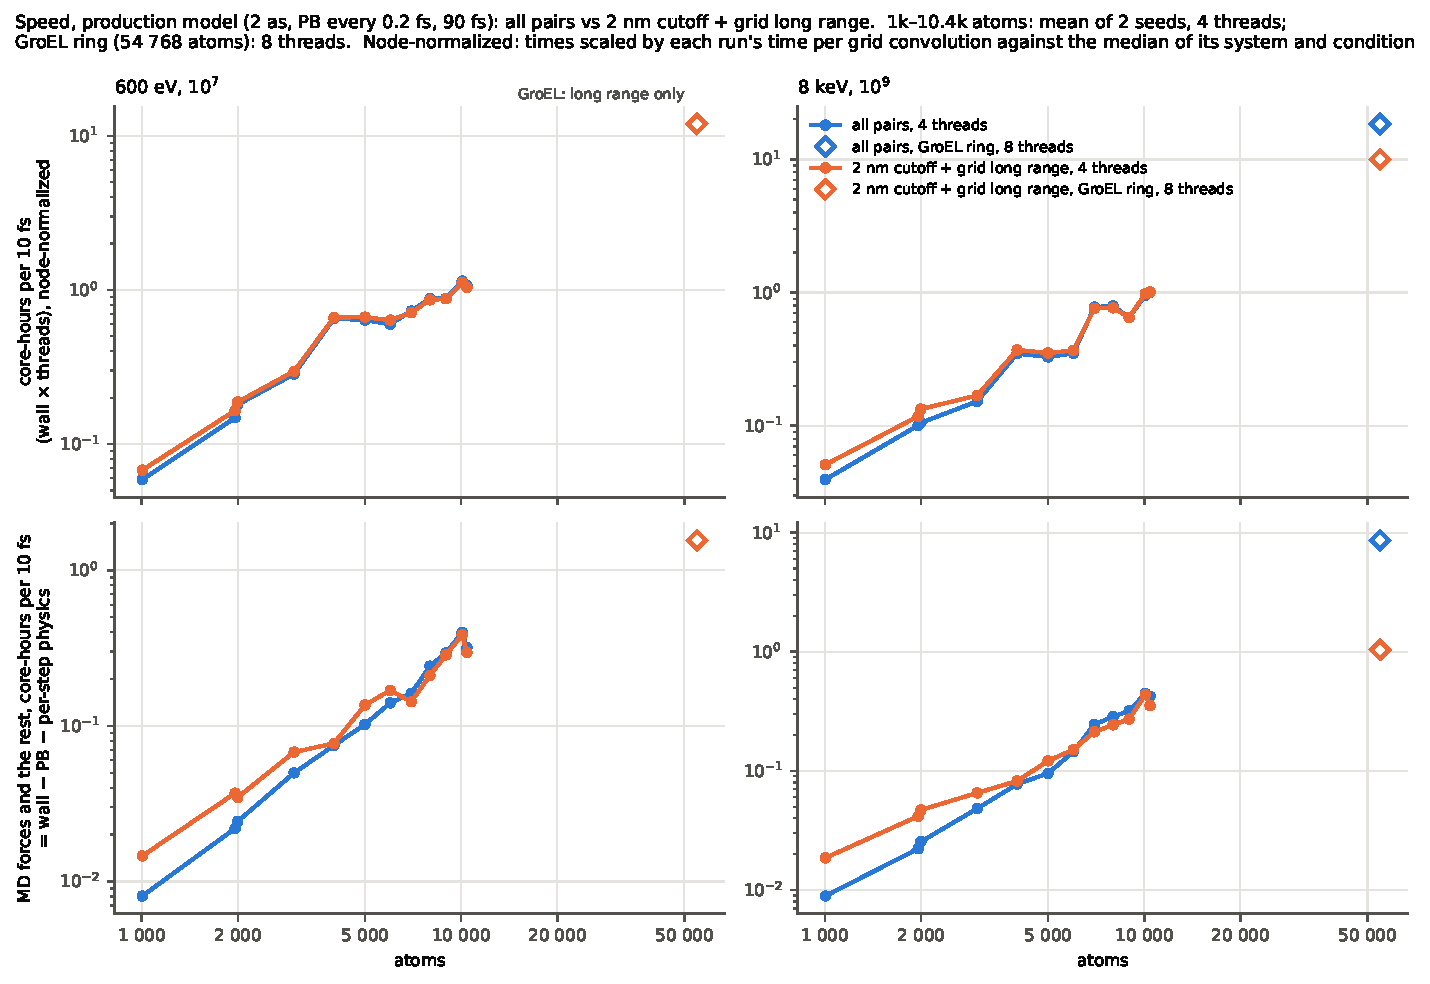
\includegraphics[width=\textwidth]{fig/size_benchmark_speed.pdf}
  \caption{Cost of the production model against system size (core-hours per 10\,fs, node-normalized): all pairs
  against the 2\,nm cutoff plus grid long range. 1k--10k atoms: 4 threads, mean of 2 seeds; GroEL: 8 threads.
  Bottom: the MD forces and the rest, without the PB solve.}
  \label{fig:speed}
\end{figure}

\chapter{Parallel runs}
\label{app:parallel}

\section{Particle decomposition}

\code{mdrun -nt N -pd} runs $N$ thread-MPI ranks with particle decomposition.
Domain decomposition is refused: it renumbers atoms into rank-local indices, and the module needs global searches over
all positions (charge transfer, the escape depth, the grid deposit).
GPUs are not supported.

\section{What runs where}

The ionization module and the PB solve run on the master rank.
To have all coordinates every step, the master gathers them over the whole ring of ranks.
During the solve the other ranks sleep on a condition variable (instead of spinning in the broadcast), and their cores
run the multithreaded FFTs (\env{GMX\_MCMD\_PBG\_FFT\_THREADS}, default the number of ranks).
The master then broadcasts the electron potential (single precision) and a few scalars, and every rank adds the cloud's
forces to its own atoms.
The MD itself (GROMACS's forces and integration) is distributed as usual.

\section{How many threads}

The PB solve dominates (50--80\,\% of the wall time) and scales with the FFT threads, the rest with the ranks.
4 threads suit 1k--10k atoms; 8 suit 50k atoms; 16 brought nothing for the GroEL ring.
For an ensemble it is usually more efficient to run many independent runs side by side than to parallelize one.

\section{Reproducibility across rank counts}

With a fixed \opt{mcmd-seed} the run is reproducible on the same number of ranks and the same build.
On a different number of ranks the electronic events are the same at first (the Monte Carlo runs on the master from one
stream), but GROMACS sums the forces in a different order, so the positions differ in the last bits ($10^{-6}$\,nm
after 2\,fs on lysozyme).
As in any MD this grows over a run: runs on different rank counts agree statistically, not bit for bit.

\chapter{Validation and limitations}
\label{app:validation}

\section{Numerical convergence}

The production settings were checked on lysozyme (1960 atoms) and 1B7U (10\,430 atoms) at 600\,eV and 8\,keV, with
several seeds per setting:
\begin{itemize}
  \item the MD step (converged at 2\,as), the PB interval (0.2\,fs), the Newton tolerance ($10^{-2}$), the box and the grid
    spacing: the charge, the escape and trapping, the radius and the ion directions are converged to within the
    seed-to-seed noise;
  \item \textbf{not converged:} the ion kinetic energy depends on the late-time smoothing --- once the grid coarsens with the
    expanding sample, the effective $s$ grows above $s_e$.
    At 600\,eV the ion kinetic energy is up to $\sim$15\,\% above that of a run with the smoothing held at $s_e$, at
    8\,keV $\sim$5\,\%.
    Compare kinetic energies between runs at equal settings.
\end{itemize}
The electron size $s_e$: charge, escape and directions are independent of it; the ion kinetic energy at 600\,eV changes
by $-15$\,\% / $+13$--19\,\% for $s_e$ = 0.20 / 0.30\,nm.

The long-range ion force (above 10\,000 atoms) leaves charge, escape and ion maps unchanged but raises the ion kinetic
energy by 2--6\,\% against all pairs (GroEL at 8\,keV: +5.3\,\%).

\section{Against a particle code}

The model was compared with XMDYN~\cite{jurek2016}, which follows every released electron as a classical particle,
run without recombination, on lysozyme (8 seeds) and 1B7U:
\begin{itemize}
  \item charge, escape, radius and ion kinetic energy agree within a few per cent at high fluence;
  \item at 600\,eV and low fluence ($10^5$) the ion kinetic energy is 11\,\% higher and the expansion starts earlier;
  \item the peak electron temperature is 25--30\,\% lower;
  \item at 8\,keV and $10^7$ the charge is half of XMDYN's (late impact ionization in a shallow well);
  \item heavy-ion maps correlate $r = 0.84$--$0.90$ with XMDYN's, against 0.88--0.93 from seed to seed; mean directions
    differ by 1.5--3$^\circ$ beyond the seed spread.
\end{itemize}

\section{Statistics}

A single run is one realization of the Monte Carlo.
A lysozyme heavy-ion map needs 3--10 seeds to correlate at $r = 0.99$ with the infinite-seed map, 1B7U one; per-atom
directions scatter by 6.5--16$^\circ$ from seed to seed.
When the start structures also differ (an ensemble of equilibrated structures, e.g.\ the ubiquitin variants), the map
needs 150--250 runs for $r = 0.99$.
The ion directions stop turning (to within 2$^\circ$) 60\,fs after the pulse peak (90\,fs at 600\,eV and low fluence).

\section{Atomic data}

The data matter: XATOM data (which match the reference photoionization cross sections) give a 15\,\% higher ion kinetic
energy at 600\,eV than the CRETIN models (whose valence cross sections are 3--12$\times$ too small), and 39\,\% higher at
1000\,eV, with the same charge to 1--2\,\% and the same directions (Section~\ref{sec:accuracy}).
The built-in screened-hydrogenic data reproduce the CRETIN models: on lysozyme at 1000\,eV the charge agrees to
0.7\,\%, the escape to 1.3\,\%, the directions within the seed noise, and the ion kinetic energy is 3.5\,\% lower.

\section{Limitations}

\begin{itemize}
  \item \textbf{Elements}: up to the M shell; elements with 4s electrons count them in M, and iodine is a placeholder.
  \item \textbf{Configurations}: shell averaged, no subshells or levels.
  \item \textbf{Electrons}: one temperature, classical mean field, escape tested at birth only
    (Chapter~\ref{ch:pb}); the ion kinetic energy depends on $s_e$ and on the late smoothing.
  \item \textbf{Not fully validated}: three-body recombination, collisional excitation, H--H charge transfer, transfer
    from heavy donors, evaporation off.
  \item \textbf{Force field}: harmonic bonds are not modified (use \code{morse = yes}; the run summary warns).
  \item \textbf{Large forces}: highly charged samples produce large forces; check that the kinetic and potential energy
    evolve smoothly, and lower \code{dt} if they do not.
  \item Tested on Linux only.
\end{itemize}

\chapter{Units, source files and history}
\label{app:misc}

\section{Units and constants}

\begin{table}[H]
\centering\small
\begin{tabular}{@{}lll@{}}
\toprule
quantity & unit & note \\ \midrule
length & nm & GROMACS \\
time & ps & GROMACS; pulse and \code{mcmd-pb-interval} in fs \\
energy (module) & eV & GROMACS uses kJ/mol: 1\,eV = 96.485\,kJ/mol \\
charge & $e$ & integer ionization charges \\
rates & s$^{-1}$ & cross sections in cm$^2$, $\langle\sigma v\rangle$ in cm$^3$\,s$^{-1}$, density in cm$^{-3}$ or nm$^{-3}$ \\
$\kc = e^2/4\pi\varepsilon_0$ & 1.43996\,eV\,nm & \code{MCMD\_COULOMB\_EV\_NM} \\
pulse FWHM / $\sigma_t$ & $2\sqrt{2\ln2} = 2.35482$ & \\
\bottomrule
\end{tabular}
\end{table}

\section{Source files}

\begin{table}[H]
\centering\small
\begin{tabularx}{\textwidth}{@{}lX@{}}
\toprule
file & content \\ \midrule
\file{src/kernel/mcionize.c} & the ionization module: Monte Carlo, charge transfer, the electron cloud, collisions,
  field ionization, output, restart state, run summary \\
\file{src/kernel/mcionize.h} & its interface to \code{md.c} \\
\file{src/kernel/atomic\_data.c}, \file{.h} & the element table, the readers of \file{Atomic\_data/}, the built-in
  screened-hydrogenic data \\
\file{src/kernel/md.c} & calls the module every step (\code{-ionize}) \\
\file{src/gmxlib/bondfree.c} & the modified bonded terms, bond breaking \\
\file{src/gmxlib/nonbonded/nonbonded.c} & the modified 1--4 Coulomb \\
\file{src/kernel/readir.c}, \file{grompp.c} & the \code{mcmd-*} options, their checks, \code{mcmd-pb-long-range = auto} \\
\file{src/gmxlib/tpxio.c}, \file{include/types/inputrec.h} & the options in the \file{.tpr} (format 76--80) \\
\file{tools/} & \file{check\_atomic\_data.py}, \file{make\_atomic\_data\_xatom.py}, \file{make\_atomic\_data\_cretin.py},
  \file{make\_collisional\_tables.py}, \file{mcmd\_output.py} \\
\file{test/regression.sh} & the regression test \\
\bottomrule
\end{tabularx}
\end{table}

\section{Version history}

\begin{description}
  \item[tpr 73--76] the original MolDStruct options as named \code{mcmd-*} parameters (formerly \code{userint},
    \code{userreal}).
  \item[tpr 77] the electron cloud and its options in the \file{.mdp} (formerly environment variables).
  \item[tpr 78] the seed and the remaining physics switches in the \file{.mdp}; \code{mcmd-pb-long-range = auto}.
  \item[tpr 79] \code{mcmd-coll-data}: Lotz's formula built in as the default; older \file{.tpr} files run as
    \code{files}.
  \item[tpr 80] \code{mcmd-atomic-data}: the screened-hydrogenic atomic data built in as the default; older
    \file{.tpr} files run with \file{./Atomic\_data} (\code{files}).
\end{description}
The model's state at this version: binary \file{transitions.bin}; the run summary with warnings; built-in
screened-hydrogenic atomic data by default, no input files; fluorescence rates corrected in both generators (earlier CRETIN-derived tables had
fluorescence rates many orders of magnitude too small and are refused by the reader).


\begin{thebibliography}{99}
\small
\bibitem{pronk2013} S.~Pronk \emph{et al.}, \emph{GROMACS 4.5: a high-throughput and highly parallel open source
molecular simulation toolkit}, Bioinformatics \textbf{29}, 845 (2013).
\bibitem{ostlin2018} C.~Östlin, N.~Tîmneanu, H.~O.~Jönsson, T.~Ekeberg, A.~V.~Martin, C.~Caleman,
\emph{Reproducibility of single protein explosions induced by X-ray lasers}, Phys.\ Chem.\ Chem.\ Phys.\ \textbf{20},
12381 (2018).
\bibitem{jurek2016} Z.~Jurek, S.-K.~Son, B.~Ziaja, R.~Santra, \emph{XMDYN and XATOM: versatile simulation tools for
quantitative modeling of X-ray free-electron laser induced dynamics of matter}, J.\ Appl.\ Cryst.\ \textbf{49}, 1048
(2016).
\bibitem{son2011} S.-K.~Son, L.~Young, R.~Santra, \emph{Impact of hollow-atom formation on coherent x-ray scattering at
high intensity}, Phys.\ Rev.\ A \textbf{83}, 033402 (2011).
\bibitem{boll2022} R.~Boll \emph{et al.}, \emph{X-ray multiphoton-induced Coulomb explosion images complex single
molecules}, Nat.\ Phys.\ \textbf{18}, 423 (2022).
\bibitem{gillespie1976} D.~T.~Gillespie, \emph{A general method for numerically simulating the stochastic time evolution
of coupled chemical reactions}, J.\ Comput.\ Phys.\ \textbf{22}, 403 (1976).
\bibitem{lotz1968} W.~Lotz, \emph{Electron-impact ionization cross-sections and ionization rate coefficients for atoms
and ions from hydrogen to calcium}, Z.\ Phys.\ \textbf{216}, 241 (1968).
\bibitem{scott2010} H.~A.~Scott, S.~B.~Hansen, \emph{Advances in NLTE modeling for integrated simulations}, High Energy
Density Phys.\ \textbf{6}, 39 (2010).
\bibitem{marchand1990} R.~Marchand, S.~Caill\'e, Y.~T.~Lee, \emph{Improved screening coefficients for the hydrogenic
ion model}, J.\ Quant.\ Spectrosc.\ Radiat.\ Transfer \textbf{43}, 149 (1990).
\bibitem{nist} A.~Kramida, Yu.~Ralchenko, J.~Reader, NIST ASD Team, \emph{NIST Atomic Spectra Database}, ionization
energies (National Institute of Standards and Technology).
\bibitem{scofield1973} J.~H.~Scofield, \emph{Theoretical photoionization cross sections from 1 to 1500 keV}, Lawrence
Livermore Laboratory report UCRL-51326 (1973).
\bibitem{krause1979} M.~O.~Krause, J.~H.~Oliver, \emph{Natural widths of atomic K and L levels, K$\alpha$ X-ray lines and
several KLL Auger lines}, J.\ Phys.\ Chem.\ Ref.\ Data \textbf{8}, 329 (1979).
\bibitem{ditmire1996} T.~Ditmire, T.~D.~Donnelly, A.~M.~Rubenchik, R.~W.~Falcone, M.~D.~Perry, \emph{Interaction of
intense laser pulses with atomic clusters}, Phys.\ Rev.\ A \textbf{53}, 3379 (1996).
\bibitem{saalmann2006} U.~Saalmann, Ch.~Siedschlag, J.~M.~Rost, \emph{Mechanisms of cluster ionization in strong laser
pulses}, J.\ Phys.\ B \textbf{39}, R39 (2006).
\bibitem{fennel2010} Th.~Fennel \emph{et al.}, \emph{Laser-driven nonlinear cluster dynamics}, Rev.\ Mod.\ Phys.\
\textbf{82}, 1793 (2010).
\bibitem{chen2016} F.~F.~Chen, \emph{Introduction to Plasma Physics and Controlled Fusion}, 3rd ed.\ (Springer, 2016).
\bibitem{nrl} J.~D.~Huba, \emph{NRL Plasma Formulary} (Naval Research Laboratory, revised editions).
\bibitem{mermin1965} N.~D.~Mermin, \emph{Thermal properties of the inhomogeneous electron gas}, Phys.\ Rev.\
\textbf{137}, A1441 (1965).
\bibitem{darden1993} T.~Darden, D.~York, L.~Pedersen, \emph{Particle mesh Ewald: An N$\cdot$log(N) method for Ewald sums
in large systems}, J.\ Chem.\ Phys.\ \textbf{98}, 10089 (1993).
\bibitem{essmann1995} U.~Essmann \emph{et al.}, \emph{A smooth particle mesh Ewald method}, J.\ Chem.\ Phys.\
\textbf{103}, 8577 (1995).
\bibitem{abramowitz1964} M.~Abramowitz, I.~A.~Stegun, \emph{Handbook of Mathematical Functions} (NBS, 1964), ch.~6.
\bibitem{birdsall1991} C.~K.~Birdsall, A.~B.~Langdon, \emph{Plasma Physics via Computer Simulation} (IOP, 1991).
\bibitem{hockney1988} R.~W.~Hockney, J.~W.~Eastwood, \emph{Computer Simulation Using Particles} (Adam Hilger, 1988).
\bibitem{hockney1970} R.~W.~Hockney, \emph{The potential calculation and some applications}, Methods Comput.\ Phys.\
\textbf{9}, 135 (1970).
\bibitem{eastwood1979} J.~W.~Eastwood, D.~R.~K.~Brownrigg, \emph{Remarks on the solution of Poisson's equation for
isolated systems}, J.\ Comput.\ Phys.\ \textbf{32}, 24 (1979).
\bibitem{frigo2005} M.~Frigo, S.~G.~Johnson, \emph{The design and implementation of FFTW3}, Proc.\ IEEE \textbf{93},
216 (2005).
\bibitem{nocedal2006} J.~Nocedal, S.~J.~Wright, \emph{Numerical Optimization}, 2nd ed.\ (Springer, 2006).
\bibitem{gould2001} N.~I.~M.~Gould, M.~E.~Hribar, J.~Nocedal, \emph{On the solution of equality constrained quadratic
programming problems arising in optimization}, SIAM J.\ Sci.\ Comput.\ \textbf{23}, 1376 (2001).
\end{thebibliography}

\end{document}
